\chapter{DENEYSEL DOĞRULAMA}
\label{chap:deney}

Önceki tezde Bölüm~5 altında ``Gerçek Zaman Uygulamaları'' başlığıyla sunulan deney düzeneği, güç donanımı, kontrol ve ölçüm kartları ile düşük güç deneyleri mevcut bölümün tarihsel kanıt kaynağını oluşturmaktadır. Kaynak Word dosyasındaki şekiller ve tablolar, aralarındaki numara ilişkisi korunarak yeniden yerleştirilmiştir. Eski Şekil~5.1--5.24 yeni tezde sırasıyla Şekil~6.1--6.24; eski Tablo~5.1--5.4 ise sırasıyla Tablo~6.1--6.4 olarak verilmektedir. Sarı etiketli içerikler önceki tezden aktarılmış, yeşil etiketli içerikler jüri talebine göre eklenen denetim veya yeterlilik değerlendirmesi olarak ayrılmıştır.

Deneylerin yeniden yapıldığı yönünde bir iddia kurulmamıştır. Görseller özgün DOCX paketinden çıkarılmış; metin, tablo ve ekran değerleri kaynak içi tutarlılık bakımından denetlenmiştir. Bölüm~\ref{chap:anahtarlama} ve Bölüm~\ref{chap:sin3} içinde incelenen klasik anahtarlama, nötr anahtar susturma ve susturma+Sin\textsuperscript{3} yöntemlerinin gerçek prototipteki düşük güç davranışı karşılaştırılmıştır.

\tezcalismanotu{D6-1 --- Deney protokolü}{Her yöntem için enerjilendirme sırası, başlangıç koşulları, sabit tutulan değişkenler, referans değerin uygulanma biçimi, kararlı duruma geçiş ölçütü, ölçüm süresi ve güvenli kapatma adımları yazılacaktır. Kayıt bulunmadan tahminî prosedür oluşturulmayacak; doğrulanamayan adımlar ``bilgi bulunamadı'' biçiminde işaretlenecektir.}

\section{Deney Düzeneği ve Güç Donanımı}

Önceki tez açıklamasına göre deney düzeneği, yaklaşık 20--25~kW güç dönüştürme kapasitesi hedeflenerek düşey bir pano üzerine bakır baralarla modüler biçimde kurulmuştur. Aynı metnin akım sensörü hesabında prototip gücü \SI{20}{\kilo\volt\ampere} olarak verilmiştir. Güç birimi ve anma değeri arasındaki fark, prototip etiketi veya tasarım dosyası bulunmadan tek bir anma değeri biçiminde birleştirilmemiştir. Raporlanan deneylerin yaklaşık \SI{2.3}{\ampere} faz akımında gerçekleştirilmesi, mevcut sonuçların anma gücü değil düşük güç doğrulaması olduğunu göstermektedir.

Şekil~\ref{fig:deney-duzenegi-genel}, varyak modülü, evirici panosu, bilgisayar ve osiloskopları aynı görünümde vermektedir. Varyak modülünde enerji bağlantıları, şalt ve koruma ekipmanları, akım transformatörleri ve AA enerji analizörü bulunduğu; üç fazın bağımsız varyaklarla ayarlanabildiği önceki tezde açıklanmıştır. Aşırı akım, kaçak akım, topraklama ve acil durdurma önlemlerinin varlığı bildirilmekle birlikte eşik ve açma süreleri kaynak kayıtlarda yer almamaktadır.

\begin{figure}[htbp]
  \centering
  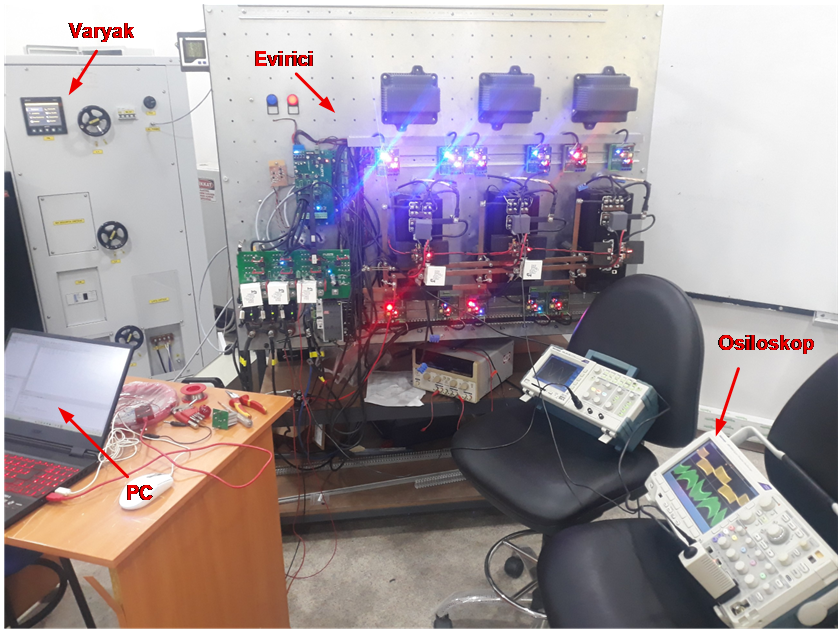
\includegraphics[width=0.95\textwidth]{deneysel/onceki_tez_sekil_5_1_deney_duzenegi.png}
  \caption{\eskitezetiketi\ Deney ve ölçme düzeneklerinin genel fotoğrafı (önceki Şekil~5.1).}
  \label{fig:deney-duzenegi-genel}
\end{figure}

Şekil~\ref{fig:deney-eski-5-2}, evirici donanımının önden genel görünümünü sunmaktadır. Üç faza ait güç modülleri, kontrol ve ölçüm kartları, DA bara bağlantıları ve yardımcı beslemeler aynı pano üzerinde görülmektedir. Genel görünüm, numaralı ayrıntıların verildiği Şekil~\ref{fig:deney-eski-5-3} için yerleşim bağlamı sağlamaktadır.

\begin{figure}[htbp]
  \centering
  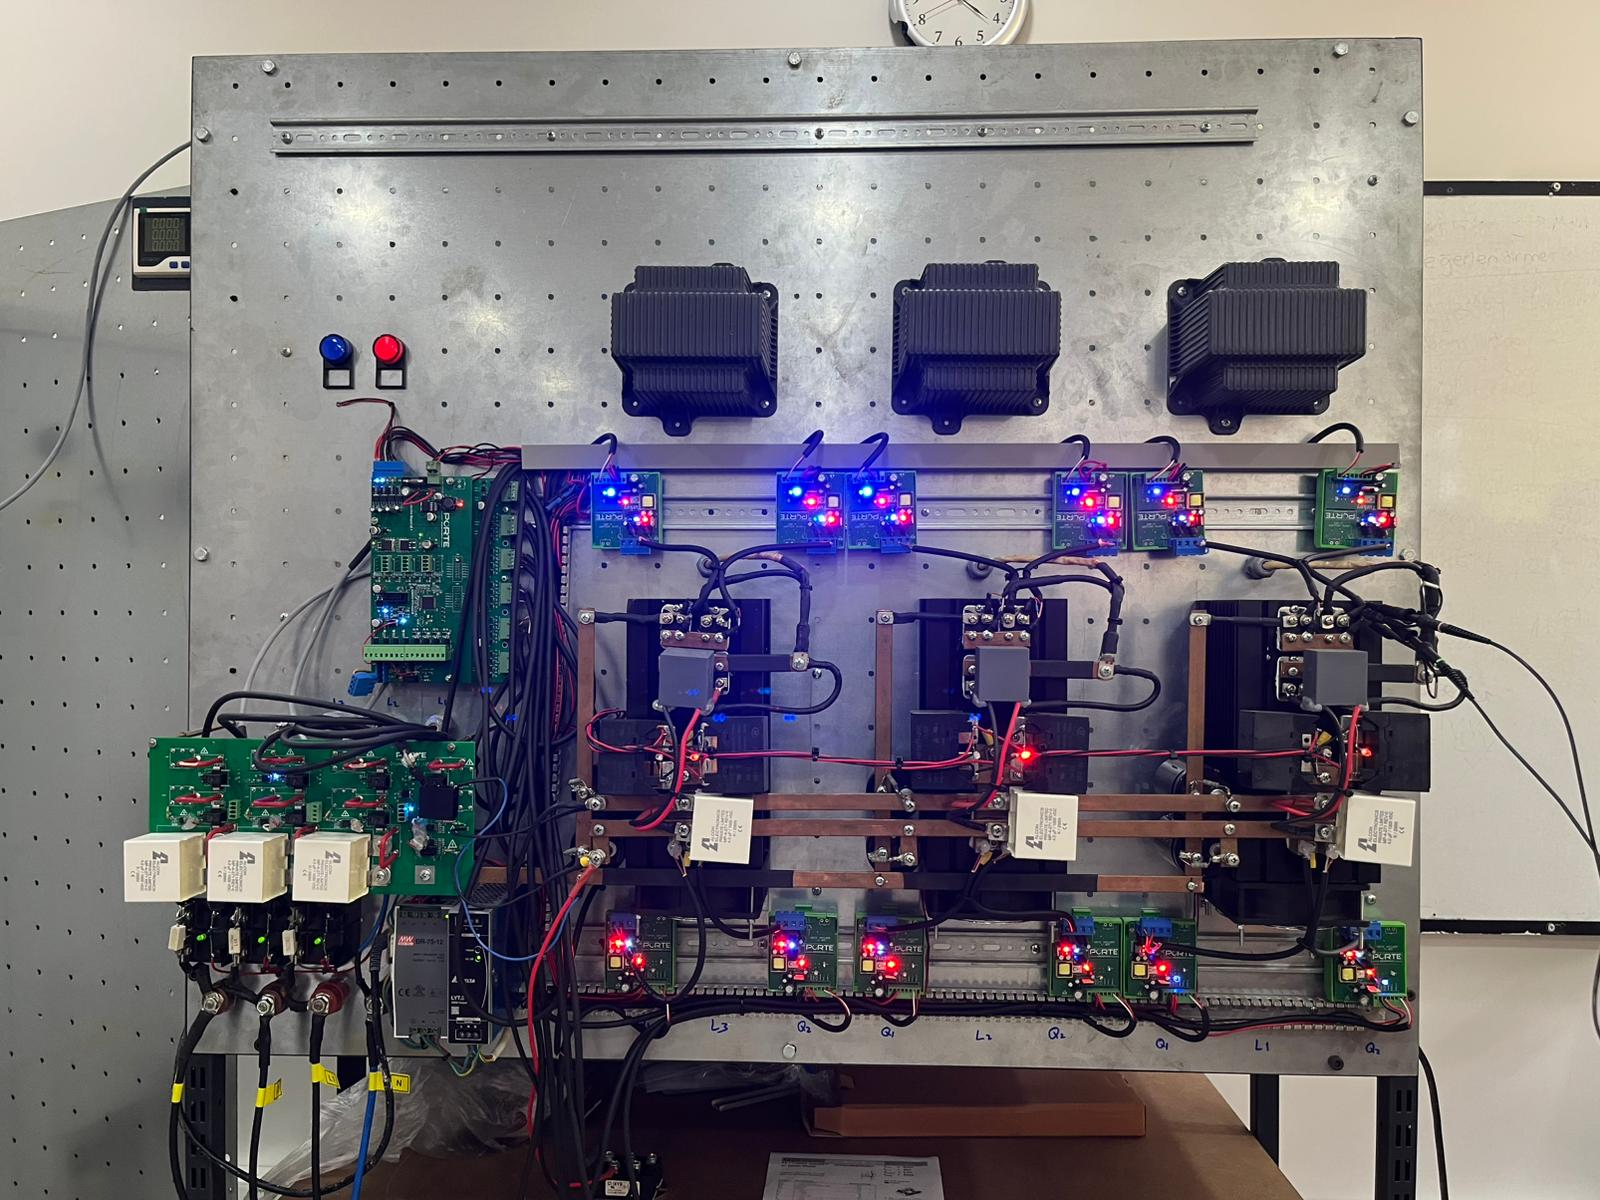
\includegraphics[width=0.88\textwidth]{deneysel/onceki_tez_sekil_5_2_evirici_donanimi.jpeg}
  \caption{\eskitezetiketi\ Evirici donanımı (önceki Şekil~5.2).}
  \label{fig:deney-eski-5-2}
\end{figure}

Şekil~\ref{fig:deney-eski-5-3} üzerindeki 1--14 numaraları doğrudan Tablo~\ref{tab:deney-alt-birimler} içindeki numaralı açıklamalara karşılık gelmektedir. Görsel ile tablo arasındaki bağ önceki tezdeki haliyle korunmuştur; bileşenler yeni işlev grupları altında birleştirilmemiştir.

\begin{figure}[htbp]
  \centering
  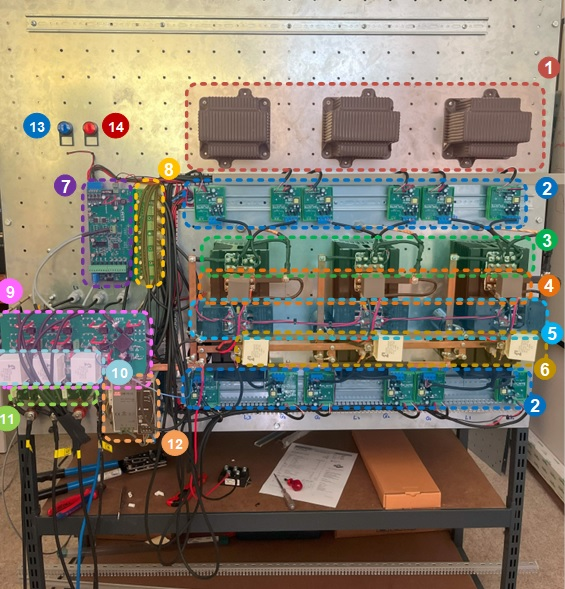
\includegraphics[width=0.72\textwidth]{deneysel/onceki_tez_sekil_5_3_donanim_alt_birimleri.jpeg}
  \caption{\eskitezetiketi\ Evirici donanımı ve alt birimlerinin numaralı tanıtımı (önceki Şekil~5.3).}
  \label{fig:deney-eski-5-3}
  \label{fig:deney-donanim-kartlar}
\end{figure}

\clearpage
\begin{table}[htbp]
  \centering
  \caption{\eskitezetiketi\ Evirici donanımı alt birimleri; önceki Tablo~5.1'in içeriği aynen korunmuştur.}
  \label{tab:deney-alt-birimler}
  \label{tab:deney-eski-5-1}
  \small
  \begin{tabularx}{0.94\textwidth}{X X}
    \toprule
    1. LCL filtrelerin L1'leri & 2. IGBT kapı sürme kartları \\
    3. Nötr IGBT'leri & 4. Boost diyotları \\
    5. Fonksiyon değiştirme röleleri & 6. Snubber kapasitörleri \\
    7. Kontrol kartı & 8. Buffer kartı \\
    9. Ölçme kartı & 10. LCL filtre C'leri \\
    11. Inrush akım röleleri & 12. Kumanda beslemeleri \\
    13. Şarj fonksiyonu lambası & 14. Deşarj fonksiyonu lambası \\
    \bottomrule
  \end{tabularx}
\end{table}

Şekil~\ref{fig:deney-eski-5-4} ve Şekil~\ref{fig:deney-eski-5-5}, aynı faz kolunun iki farklı açıdan çekilmiş ayrıntılarını göstermektedir. Her iki görseldeki 1--8 numaraları Tablo~\ref{tab:deney-eski-5-2} ile birlikte okunmalıdır. İki görüntünün ayrı tutulması; boost diyotları, fonksiyon değiştirme röleleri, DA bara ve snubber kapasitörleri, soğutma düzeni, sürücü kartı ve $L_1$ bobininin fiziksel konumunu kaybetmeden izlemeyi sağlamaktadır.

\begin{figure}[htbp]
  \centering
  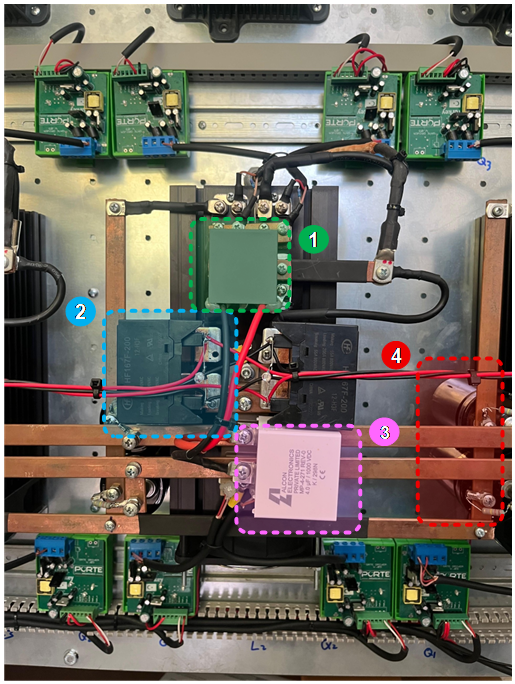
\includegraphics[height=0.68\textheight]{deneysel/onceki_tez_sekil_5_4_faz_donanimlari_1.png}
  \caption{\eskitezetiketi\ Eviricinin bir fazına ait donanımlar, birinci görünüm (önceki Şekil~5.4).}
  \label{fig:deney-eski-5-4}
\end{figure}

\begin{figure}[htbp]
  \centering
  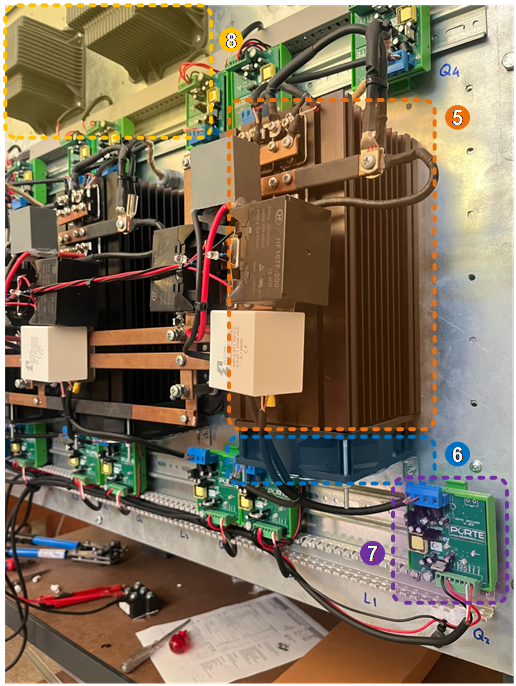
\includegraphics[height=0.68\textheight]{deneysel/onceki_tez_sekil_5_5_faz_donanimlari_2.png}
  \caption{\eskitezetiketi\ Eviricinin bir fazına ait donanımlar, ikinci görünüm (önceki Şekil~5.5).}
  \label{fig:deney-eski-5-5}
\end{figure}

\clearpage
\begin{table}[htbp]
  \centering
  \caption{\eskitezetiketi\ Şekil~\ref{fig:deney-eski-5-4} ve Şekil~\ref{fig:deney-eski-5-5}'teki donanıma ait komponentler; önceki Tablo~5.2'nin içeriği aynen korunmuştur.}
  \label{tab:deney-eski-5-2}
  \small
  \begin{tabularx}{0.94\textwidth}{X X}
    \toprule
    1. Boost diyotları ve kondansatörü & 2. Fonksiyon değiştirme röleleri \\
    3. Snubber kondansatörleri & 4. DA bara elektrolitik kondansatörleri \\
    5. IGBT soğutucu (99 AS) & 6. Yüksek devirli soğutma fanı \\
    7. IGBT kapı sürme kartı & 8. LCL filtre L1 bobini \\
    \bottomrule
  \end{tabularx}
\end{table}

Şekil~\ref{fig:deney-eski-5-6}, evirici giriş devresini ve 1--6 ile işaretlenmiş yardımcı donanımları göstermektedir. Numaraların karşılığı Tablo~\ref{tab:deney-eski-5-3}'te korunmuştur. Giriş bölümünün ayrı verilmesi; inrush röleleri, sigorta, yardımcı kaynaklar, EMI filtresi, kontrol kartı ve buffer kartının güç katıyla bağlantısını görünür kılmaktadır.

\begin{figure}[htbp]
  \centering
  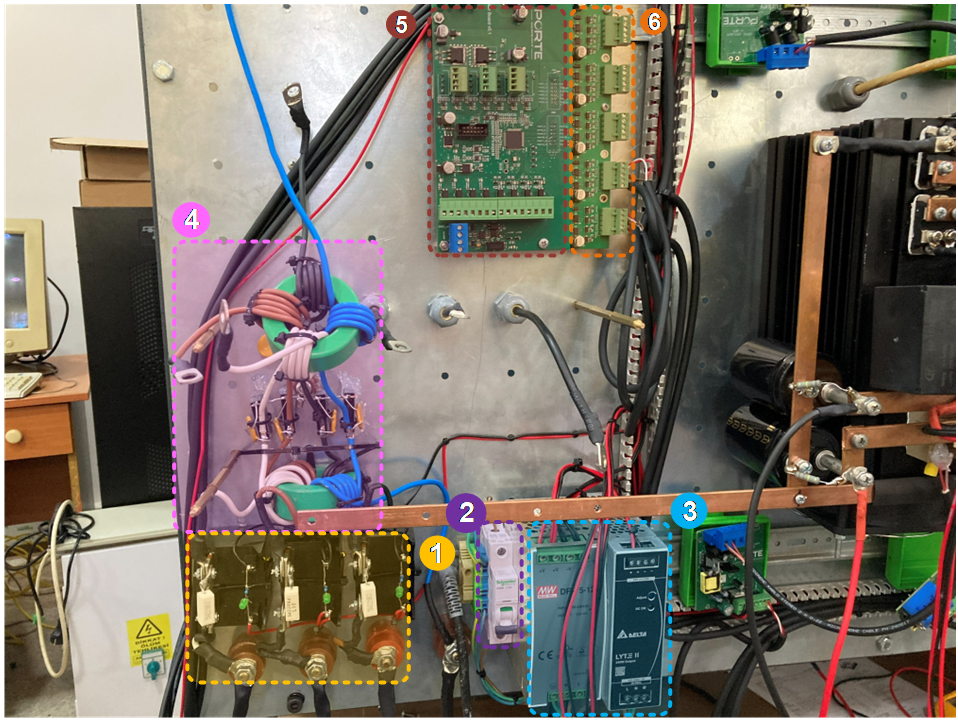
\includegraphics[width=0.94\textwidth]{deneysel/onceki_tez_sekil_5_6_giris_devresi.png}
  \caption{\eskitezetiketi\ Evirici giriş devresinin detay görüntüsü (önceki Şekil~5.6).}
  \label{fig:deney-eski-5-6}
\end{figure}

\clearpage
\begin{table}[htbp]
  \centering
  \caption{\eskitezetiketi\ Evirici donanımının giriş kısmına ait komponentler; önceki Tablo~5.3'ün içeriği aynen korunmuştur.}
  \label{tab:deney-eski-5-3}
  \small
  \begin{tabularx}{0.94\textwidth}{X X}
    \toprule
    1. Inrush akım röleleri & 2. Evirici açma kapama sigortası \\
    3. 12 V--24 V güç kaynakları & 4. EMI filtre \\
    5. Kontrol kartı & 6. Buffer kartı \\
    \bottomrule
  \end{tabularx}
\end{table}

\section{Kontrol Kartı, Buffer Kartı ve Kapı Sürücüsü}

Şekil~\ref{fig:deney-eski-5-7}, önceki tezde numaralandırılmış kontrol ve buffer kartlarını göstermektedir. Kontrol kartında RS485 haberleşme birimi, optoizole giriş/çıkışlar, DA bara ve akım ölçüm dönüştürme devreleri, PIC32MK ailesi mikrodenetleyici, lineer regülatörler ve röle/fan çıkış katları bulunmaktadır. Buffer kartı, mikrodenetleyicinin \SI{3.3}{\volt} single-ended PWM işaretlerini diferansiyel sinyal çiftlerine dönüştürmek ve uzun ekranlı kablolarda ortak-mod gürültü etkisini azaltmak amacıyla kullanılmıştır.

\eskitezetiketi\ Kaynak metindeki fotoğraf numaraları işlevleriyle birlikte korunmuştur: (1) RS485 haberleşme; (2)--(3) optoizole giriş ve çıkışlar; (4) diferansiyel DA bara gerilimini single-ended biçime dönüştüren ölçüm katı; (5) ölçüm, haberleşme ve kontrol algoritmalarını yürüten PIC32MK mikrodenetleyici; (6) akım ölçüm dönüştürme katı; (7) \SI{5}{\volt} lineer regülatörler; (8) röle ve fanlar için MOSFET güç çıkışları; (9) \SI{9}{\volt} anahtarlamalı regülatör; (10) PWM buffer kartının \SI{9}{\volt} beslemesi ve (11) single-ended PWM işaretlerini diferansiyel çiftlere dönüştüren kat. Böylece Şekil~\ref{fig:deney-eski-5-7} yalnız genel kart fotoğrafı değil, önceki tezdeki 1--11 işlev eşlemesinin görsel karşılığı olarak kullanılmaktadır.

\begin{figure}[htbp]
  \centering
  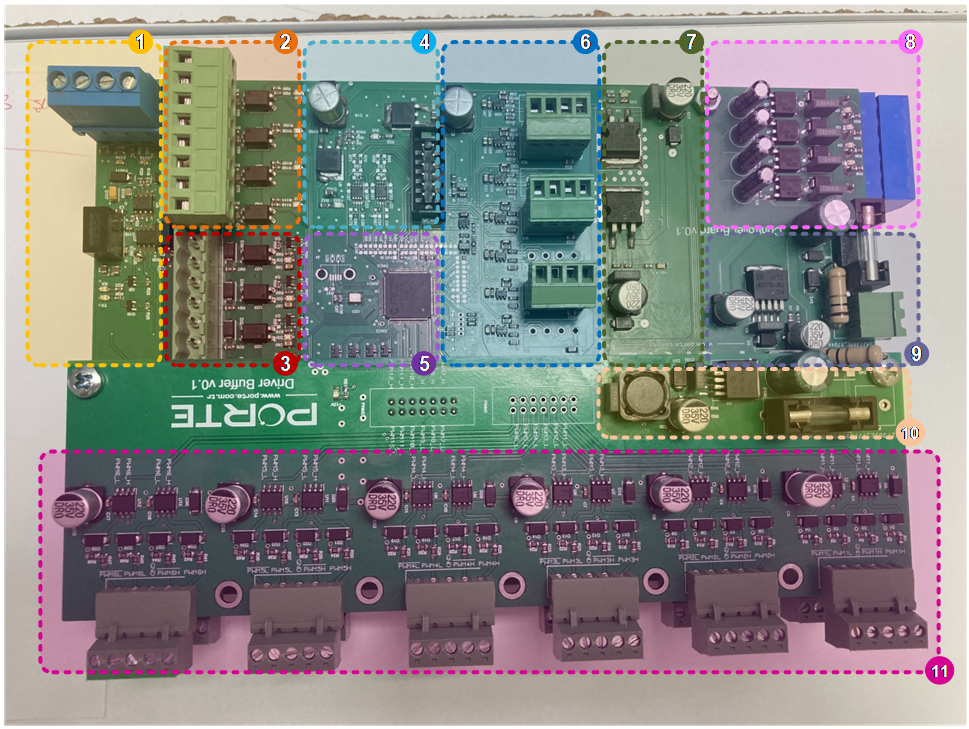
\includegraphics[width=0.90\textwidth]{deneysel/onceki_tez_sekil_5_7_kontrol_buffer.png}
  \caption{\eskitezetiketi\ Kontrol kartı ve buffer kartının numaralı fotoğrafı (önceki Şekil~5.7).}
  \label{fig:deney-eski-5-7}
\end{figure}

Önceki tezde PWM1--PWM6 kanallarının yüksek ve alçak işaretlerinin buffer kartında diferansiyel çiftlere dönüştürüldüğü, yaklaşık \SI{12}{\volt} genlikte ve tek yönlü iletim amacıyla H-köprü tabanlı sürme çözümü kullanıldığı açıklanmıştır. Gerçek PWM kaynak kodu, ölü zaman, minimum darbe süresi ve çıkış gecikmeleri bulunmadığından söz konusu zincirin zamanlama performansı henüz yeniden doğrulanamamıştır.

Şekil~\ref{fig:deney-eski-5-8}, ADuM4135 tabanlı olduğu bildirilen IGBT kapı sürme kartını göstermektedir. Diferansiyel giriş, desatürasyon koruması, aktif Miller kenetleme ve düşük gerilim kilitleme özellikleri sürücü seçim gerekçeleri olarak verilmiştir. Bütün sürücülerden gelen FAULT çıkışlarının kontrol kartında toplandığı ve ortak RESET işaretinin sürücülere paralel dağıtıldığı kaynak metinde belirtilmiştir.

\begin{minipage}{\linewidth}
\eskitezetiketi\ Önceki tez, diferansiyel girişin uzun PWM hatlarındaki ortak-mod gürültüsüne karşı bağışıklık sağladığını; desatürasyon korumasının aşırı akımda IGBT komutunu donanımsal olarak kestiğini ve aktif Miller kenetlemenin yanlış iletime geçme riskini azalttığını açıklamaktadır. FAULT bilgisinin optoizole giriş üzerinden yazılıma taşınması ve ortak RESET hattıyla bütün sürücülerin yeniden etkinleştirilmesi, donanım koruması ile denetim yazılımı arasındaki hata yönetim zincirini oluşturmaktadır. Tedarik, stok ve maliyet etkenleri de ADuM4135 seçiminde pratik ölçütler olarak bildirilmiştir.
\end{minipage}

\begin{figure}[htbp]
  \centering
  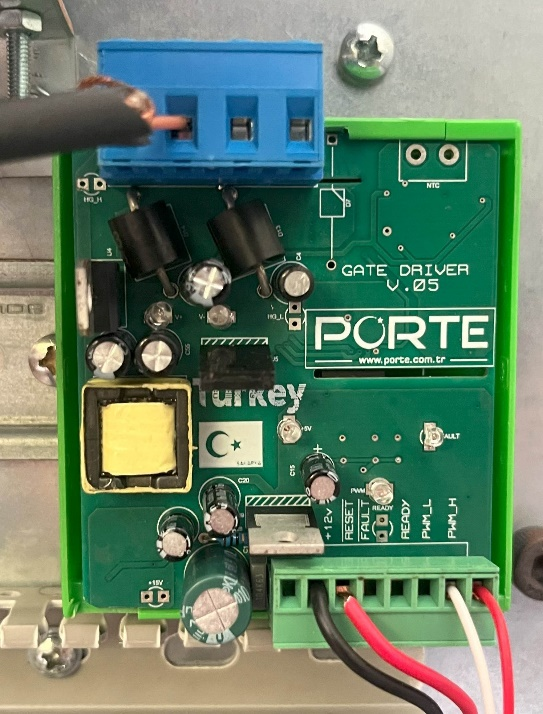
\includegraphics[height=0.64\textheight]{deneysel/onceki_tez_sekil_5_8_igbt_surucu.jpeg}
  \caption{\eskitezetiketi\ IGBT kapı sürme devresi fotoğrafı (önceki Şekil~5.8).}
  \label{fig:deney-eski-5-8}
\end{figure}

\clearpage
\section{Gerilim ve Akım Ölçme Devreleri}

Faz--nötr gerilimleri ile pozitif ve negatif DA bara gerilimlerinin AMC1200 tabanlı izole ölçüm devreleriyle alındığı önceki tezde açıklanmıştır. AMC1200 için diferansiyel çıkış ofseti yaklaşık \SI{1.3}{\volt}, çıkış aralığı 0--\SI{2.6}{\volt} ve gerilim kazancı 8 olarak verilmiştir. Söz konusu değerlere göre girişte izin verilen en yüksek genlik \SI{162.5}{\milli\volt} olarak hesaplanmış; faz ve DA bara ölçümleri için ayrı gerilim bölücüler kullanılmıştır. Kaynak metin faz ölçüm sınırını anlık yaklaşık \SI{387}{\volt}, DA bara giriş ayarını \SI{470}{\volt} DA olarak bildirmektedir.

\eskitezetiketi\ Mikrodenetleyicideki yedi ADC kanalının üçü faz--nötr gerilimlerine, ikisi ise pozitif ve negatif DA bara gerilimlerine ayrılmıştır. Faz ölçümleri AMC1200 çıkışlarından ekranlı kabloyla diferansiyel olarak taşınmış ve RC anti-aliasing filtrelerinden geçirilmiştir. DA bara kanallarında diferansiyel işaretlerin enstrümantasyon yükselteciyle işlenip \SI{1.3}{\volt} ofset eklenerek single-ended biçime dönüştürüldüğü açıklanmıştır. Kaynakta verilen 12 bit ADC gösterimi, diferansiyel sayısal aralığı yaklaşık $-2047$ ile $+2048$ arasında tanımlamaktadır.

Dört telli T-tipi yapıda nötr noktasının kayması, iki DA bara kondansatörünün gerilimlerini eşitsizleştirebileceğinden pozitif ve negatif bara kanalları sürekli izlenmiştir. Kaynak metne göre eşik aşımında mikrodenetleyici FAULT üretip PWM çıkışlarını kesmektedir. AMC1200 giriş beslemesi, \SI{5}{\volt}/\SI{5}{\volt} ve \SI{1}{\watt} değerli RFM-0505S izole dönüştürücü ile sağlanmış; dönüştürücü çıkışındaki regülasyon zayıflığını azaltmak amacıyla TCR2EF250 düşük gerilim düşümlü regülatör kullanılmıştır. Söz konusu ayrıntılar ölçüm zincirinin yalnız ölçekleme değil, izolasyon ve nötr nokta koruması görevlerini de üstlendiğini göstermektedir.

Akım ölçümünde HLSR 20-P/SP33 Hall etkili sensör kullanılmıştır. Sensör kazancı \SI{23}{\milli\volt\per\ampere}, referans gerilimi \SI{1.3}{\volt} ve hesaplanan simetrik en yüksek akım yaklaşık \SI{56.5}{\ampere} tepe ya da \SI{39.9}{\ampere} RMS'tir. Prototip için faz başına yaklaşık \SI{30}{\ampere} RMS ve yüzde 20 toleransla \SI{36}{\ampere} RMS tasarım değeri verilmiştir. Hesapların gerçek direnç toleransları, ADC kalibrasyonu ve sensör sıcaklık sapmasıyla yeniden doğrulanması gerekmektedir.

Ani faz ve kondansatör akımlarının sınırlandırılması amacıyla kullanılan pencere karşılaştırıcı devre Şekil~\ref{fig:deney-eski-5-9}'da verilmiştir. Devrede üst eşik \SI{2.0}{\volt}, alt eşik \SI{0.6}{\volt} ve referans \SI{1.3}{\volt} olarak ayarlanmıştır. \SI{0.7}{\volt} eşik farkı, \SI{23}{\milli\volt\per\ampere} sensör kazancıyla yaklaşık \SI{30.4}{\ampere} akıma karşılık gelmektedir. Eşik dışına çıkıldığında FAULT işaretinin kontrol kartında harici kesme oluşturarak PWM çıkışlarını kesmesi amaçlanmıştır.

\begin{figure}[htbp]
  \centering
  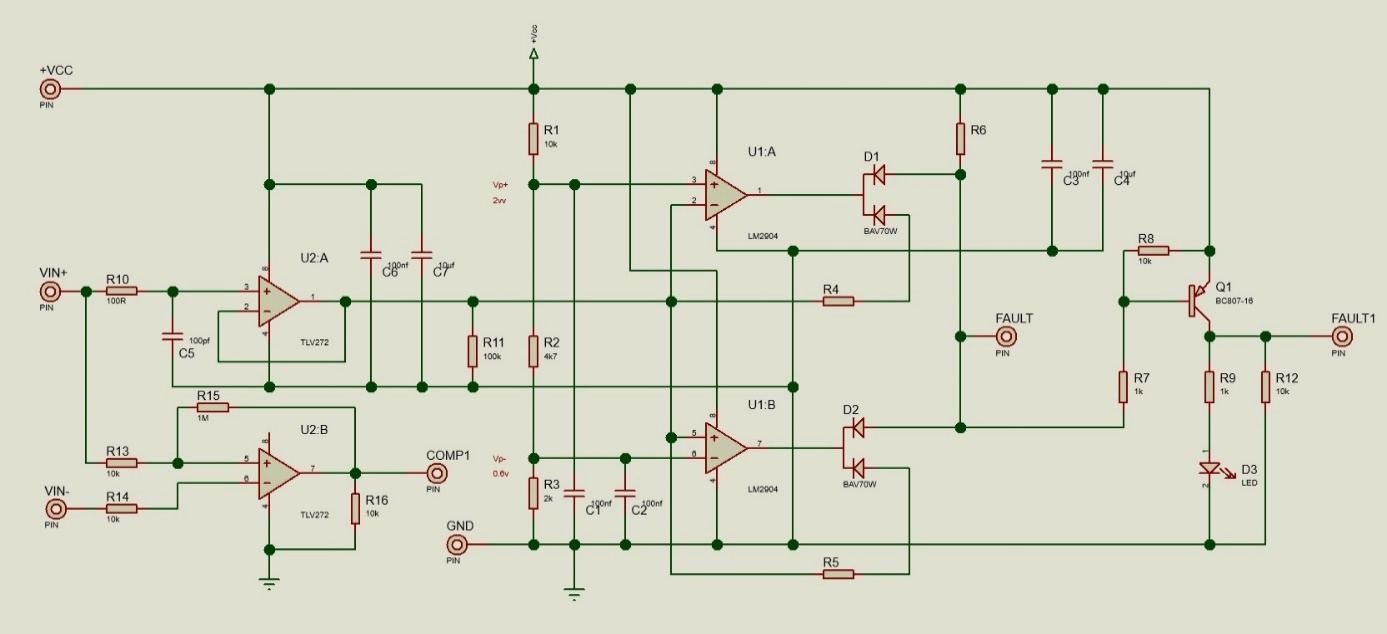
\includegraphics[width=0.96\textwidth]{deneysel/onceki_tez_sekil_5_9_pencere_karsilastirici.jpeg}
  \caption{\eskitezetiketi\ Pencere karşılaştırıcı devresi (önceki Şekil~5.9).}
  \label{fig:deney-eski-5-9}
\end{figure}

Şekil~\ref{fig:deney-eski-5-10}, harici bir deneme kartının DAC çıkışıyla uygulanan giriş işareti ve pencere karşılaştırıcının FAULT çıkışını göstermektedir. Cursor1 ve Cursor2 seviyeleri sırasıyla \SI{2.0}{\volt} ve \SI{0.6}{\volt} olarak ayarlanmış; giriş sınırların dışına çıktığında CH2 işaretinin lojik sıfıra indiği gözlenmiştir. Kayıt, koruma mantığının işlevsel örneğidir; gecikme süresi ve gerçek kısa-devre kesme enerjisi aynı görüntüden çıkarılamamaktadır.

\begin{figure}[htbp]
  \centering
  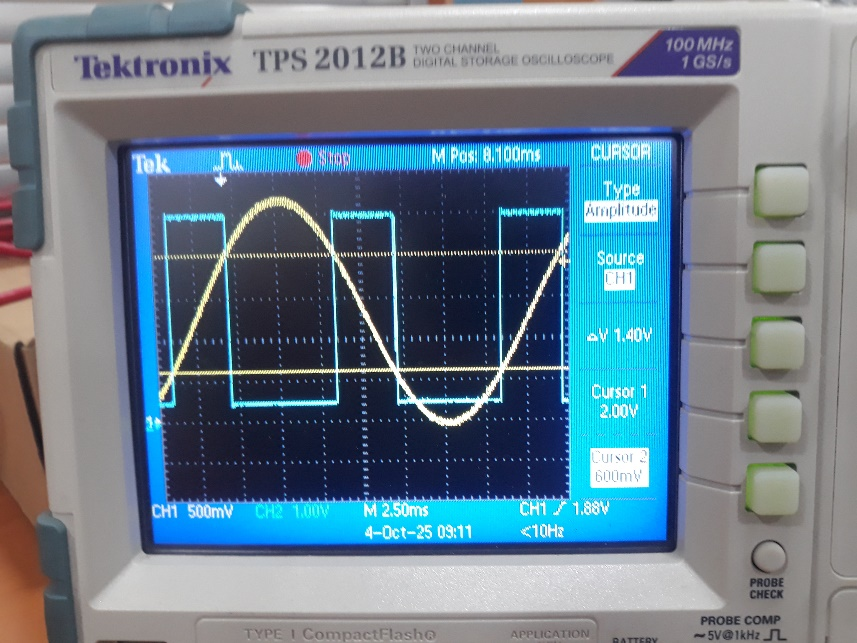
\includegraphics[width=0.88\textwidth]{deneysel/onceki_tez_sekil_5_10_pencere_dalga.jpeg}
  \caption{\eskitezetiketi\ Pencere karşılaştırıcı giriş ve çıkış gerilim dalga şekilleri (önceki Şekil~5.10).}
  \label{fig:deney-eski-5-10}
\end{figure}

Şekil~\ref{fig:deney-eski-5-11}, HLSR akım sensörleri, AMC1200 izole ölçüm kanalları ve akım probu bağlantı iletkenlerini içeren ölçüm kartını göstermektedir. Kart üzerindeki \SI{4}{\milli\metre\squared} kesitli ters-U biçimli iletkenler; faz başına $L_1$ akımı, kondansatör akımı ve faz akımının ayrı ayrı osiloskop probuyla ölçülmesini sağlamaktadır. TLV431 referansları ve MC33269 regülatörleri ölçüm beslemesi ile \SI{1.3}{\volt} ofset üretiminde kullanılmıştır.

\begin{figure}[htbp]
  \centering
  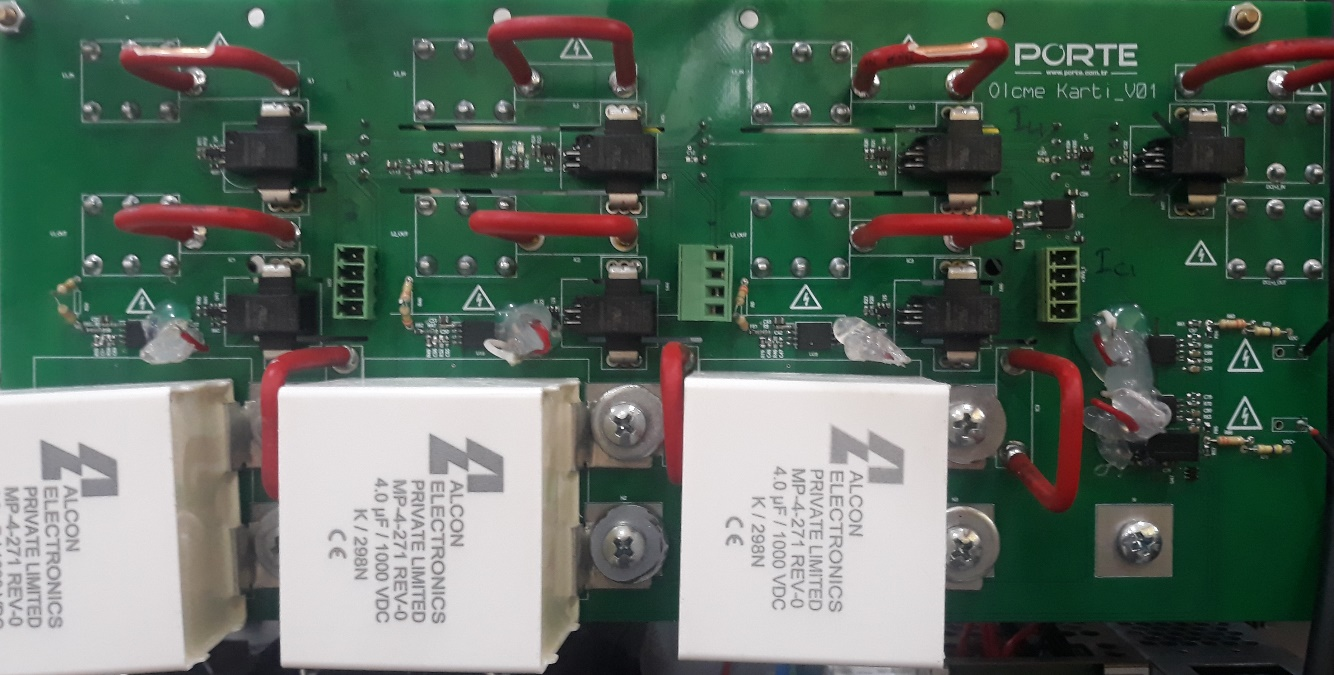
\includegraphics[width=0.96\textwidth]{deneysel/onceki_tez_sekil_5_11_olcum_karti.jpeg}
  \caption{\eskitezetiketi\ Ölçüm kartı (önceki Şekil~5.11).}
  \label{fig:deney-eski-5-11}
\end{figure}

\section{DA ve AA Güç Analizörleri}

DA bara gerilimi, akımı ve gücü Accuenergy AcuDC240 analizörüyle ölçülmüştür. Önceki tez, cihazın akım ve gerilim ölçümleri için yüzde 0,2; güç ve enerji ölçümleri için yüzde 0,5 hata toleransı verdiğini bildirmektedir. Şekil~\ref{fig:deney-eski-5-12}(a) cihazın pano üzerindeki konumunu, Şekil~\ref{fig:deney-eski-5-12}(b) üretici dokümanındaki şönt bağlantısını göstermektedir.

\begin{figure}[htbp]
  \centering
  \begin{subfigure}[t]{0.46\textwidth}
    \centering
    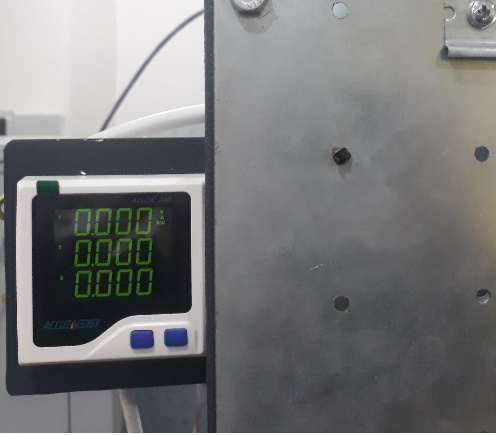
\includegraphics[width=\linewidth]{deneysel/onceki_tez_sekil_5_12a_acudc240.jpeg}
    \caption{Evirici donanımı üzerindeki AcuDC240.}
  \end{subfigure}\hfill
  \begin{subfigure}[t]{0.50\textwidth}
    \centering
    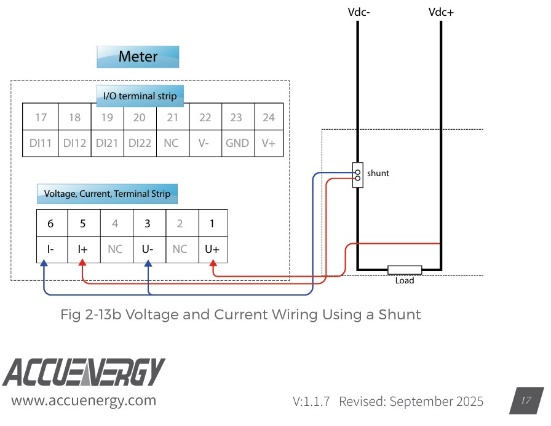
\includegraphics[width=\linewidth]{deneysel/onceki_tez_sekil_5_12b_acudc240_baglanti.jpeg}
    \caption{DA analizörü ve şönt bağlantı şekli.}
  \end{subfigure}
  \caption{\eskitezetiketi\ AcuDC240 DA bara analizörü ve bağlantısı (önceki Şekil~5.12).}
  \label{fig:deney-eski-5-12}
\end{figure}

Prototipte şönt direnci DA baranın negatif terminaline bağlanarak alçak-taraf akım ölçümü yapılmıştır. Şekil~\ref{fig:deney-eski-5-13}, \SI{20}{\ampere}/\SI{60}{\milli\volt} şönt direncin fiziksel bağlantısını göstermektedir. Şöntün ölçüm uçlarının koaksiyel ve ekranlı kabloyla analizöre taşındığı; DA gerilim girişinde ise yüksek izolasyon dayanımlı kablo kullanıldığı kaynak metinde belirtilmiştir.

\begin{figure}[htbp]
  \centering
  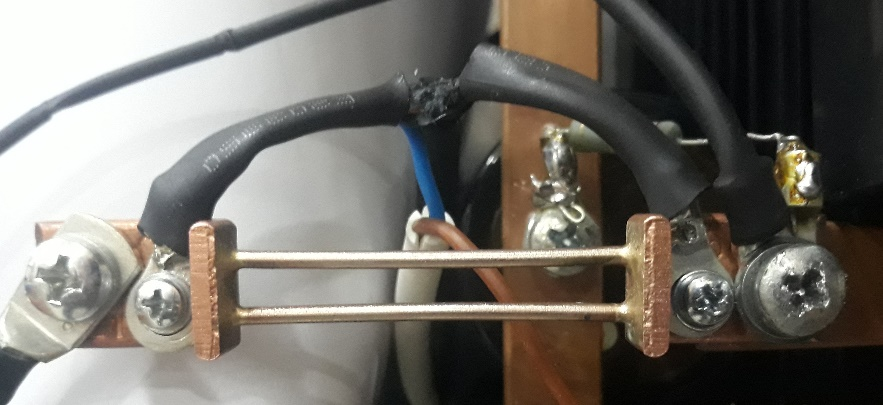
\includegraphics[width=0.94\textwidth]{deneysel/onceki_tez_sekil_5_13_sont_baglanti.jpeg}
  \caption{\eskitezetiketi\ \SI{20}{\ampere}--\SI{60}{\milli\volt} şönt direnç bağlantısı (önceki Şekil~5.13).}
  \label{fig:deney-eski-5-13}
\end{figure}

AA tarafta Entes EMK-01 analizörü ve 50/5 oranlı, \SI{5}{\volt\ampere}, Class~0.1 akım transformatörleri kullanılmıştır. Üç faz ve nötr hattı için dört akım transformatörünün bağlandığı; faz--nötr gerilimleri, faz/nötr akımları, aktif ve reaktif güç ile toplam THD değerlerinin Modbus RTU üzerinden okunduğu açıklanmıştır. Şekil~\ref{fig:deney-eski-5-14}(a) analizörü, Şekil~\ref{fig:deney-eski-5-14}(b) üreticinin bağlantı düzenini vermektedir.

\begin{figure}[htbp]
  \centering
  \begin{subfigure}[t]{0.43\textwidth}
    \centering
    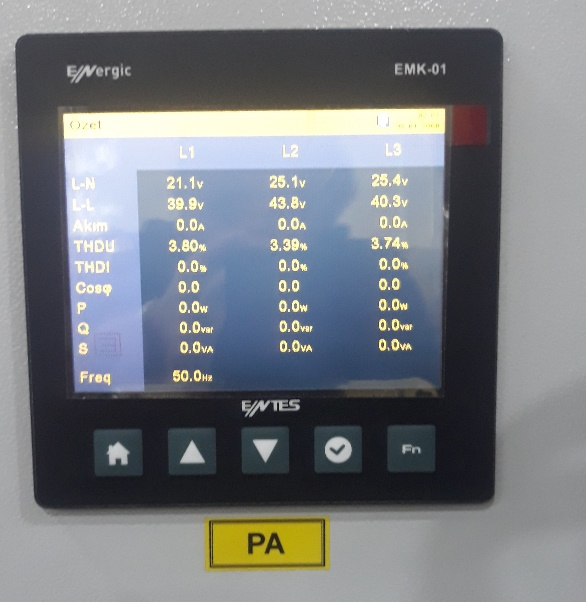
\includegraphics[width=\linewidth]{deneysel/onceki_tez_sekil_5_14a_emk01.jpeg}
    \caption{EMK-01 AA analizörü.}
  \end{subfigure}\hfill
  \begin{subfigure}[t]{0.53\textwidth}
    \centering
    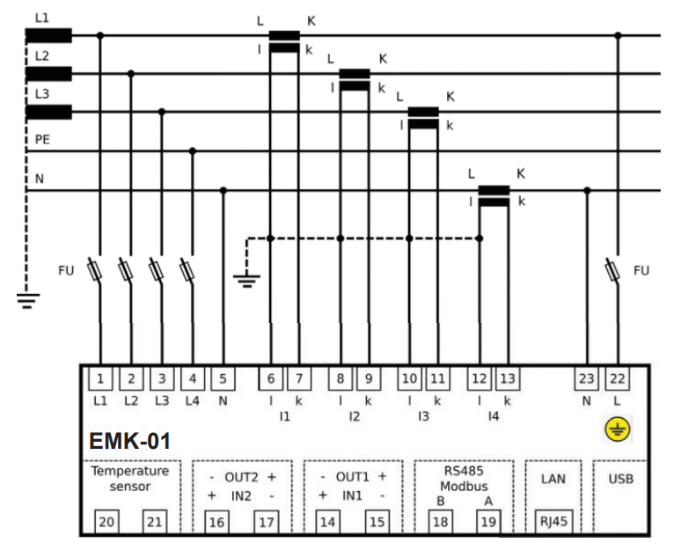
\includegraphics[width=\linewidth]{deneysel/onceki_tez_sekil_5_14b_emk01_baglanti.png}
    \caption{Üretici tarafından önerilen bağlantı şekli.}
  \end{subfigure}
  \caption{\eskitezetiketi\ EMK-01 AA analizörü ve bağlantısı (önceki Şekil~5.14; kaynak başlığındaki ``Şekil 14'' yazımı bölüm numarasıyla düzeltilmiştir).}
  \label{fig:deney-eski-5-14}
\end{figure}

\section{PC Ana Kumanda Yazılımı ve Veri Toplama}

PC ana kumanda yazılımı; EMK-01, AcuDC240 ve kontrol kartından RS485/Modbus RTU üzerinden veri almak, anlık değerleri grafikleştirmek ve verim hesabına temel oluşturmak amacıyla geliştirilmiştir. Şekil~\ref{fig:deney-pc-arayuzu}, yazılımın özgün arayüzünü göstermektedir. Kaynak metin bir veri çevriminin yaklaşık \SI{1}{\second} sürdüğünü, önce DA analizörünün ve en fazla yaklaşık \SI{50}{\milli\second} sonra AA analizörünün okunduğunu bildirmektedir. Söz konusu yapı kararlı durum eğilimleri için kullanılabilir; hızlı geçici rejimlerin tam eşzamanlı karşılaştırılması için yeterli değildir.

\eskitezetiketi\ Haberleşme hızı cihazların izin verdiği en yüksek değer olarak 38400 baud seçilmiş; veri sırası DA analizörü, AA analizörü ve kontrol kartı biçiminde kurulmuştur. Yazılımın karşılaştırma seti verim, THD, güç faktörü, faz akımı, faz--nötr gerilimi ve DA bara geriliminden oluşmaktadır. Önceki tezde ``kontrolör kullanılmadığı'' ifadesi yer alırken osiloskop açıklamalarında DAC üzerinden ``kontrolör çıkışı'' adı kullanılmaktadır. İki ifade arasındaki anlam farkı kaynak kod olmadan çözülemediğinden, kontrol yapısına ilişkin kesin yorum Bölüm~\ref{chap:sin3} içindeki doğrulama maddesi olarak korunmuştur.

\begin{figure}[htbp]
  \centering
  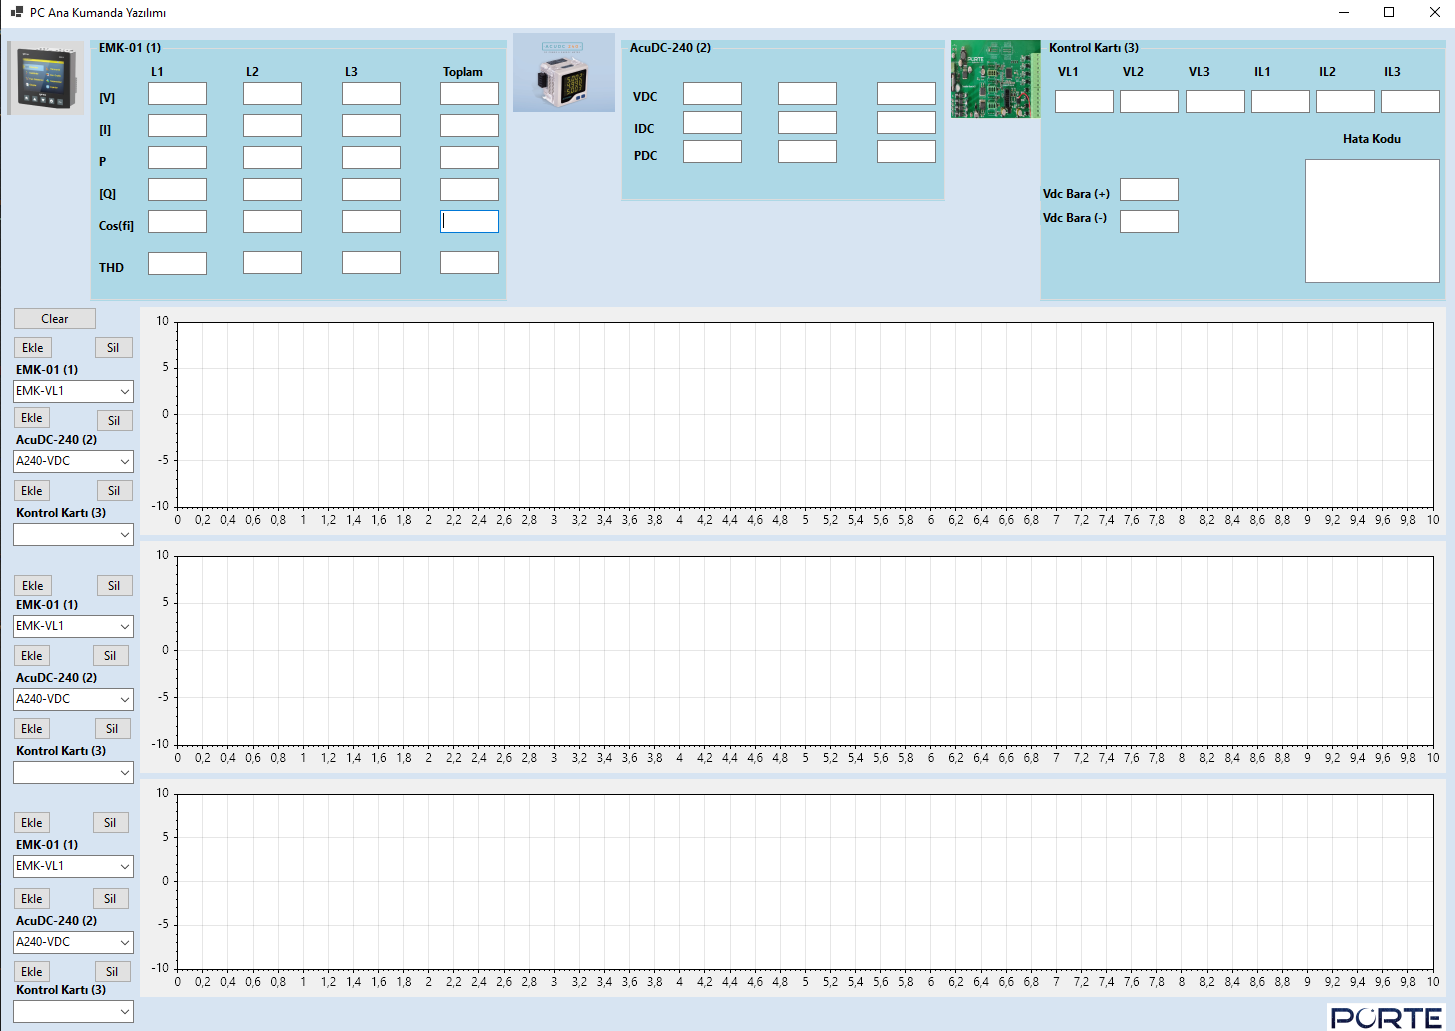
\includegraphics[width=0.98\textwidth]{deneysel/onceki_tez_sekil_5_15_pc_arayuzu.png}
  \caption{\eskitezetiketi\ Haberleşme sistemi arayüz tasarımı (önceki Şekil~5.15).}
  \label{fig:deney-pc-arayuzu}
  \label{fig:deney-eski-5-15}
\end{figure}

Önceki tezde ortak hedef çalışma koşulu; DA bara gerilimi yaklaşık \SI{400}{\volt}, faz--nötr gerilimi yaklaşık \SI{130}{\volt}, faz akımı yaklaşık \SI{2.3}{\ampere} ve birim güç faktörüne yakın işletim olarak tanımlanmıştır. Gerçek ekran ve metin kayıtları yöntemler arasında farklı DA bara ve faz gerilimleri bulunduğunu göstermektedir. Verim, THD ve ters akım ölçütleri Eşitlik~\eqref{eq:verim-tanimi}, Eşitlik~\eqref{eq:thd-rmse-tanimlari} ve Eşitlik~\eqref{eq:ters-akim-anahtarlama-olcutleri} ile ilişkilendirilmiştir.

\tezcalismanotu{D6-2 --- Ham veri izlenebilirliği}{Her PC/Modbus ve osiloskop kaydı için deney tarihi, yöntem, çalışma noktası, özgün dosya adı, kanal adı, fiziksel birim, sensör/prob oranı, örnekleme hızı ve kullanılan analiz penceresi tek bir koşu kimliğiyle kaydedilecektir. Yalnız ekran görüntüsü bulunan sonuçlar ham veri elde edilene kadar tarihsel destekleyici kanıt sayılacaktır.}

\section{Klasik Anahtarlama Modu Deney Kayıtları}

Klasik yöntemde bütün anahtarların tamamlayıcı sürüldüğü ve düşük akımda senkron-buck benzeri ters akım yolunun açık kaldığı Bölüm~\ref{chap:anahtarlama} içinde açıklanmıştır. Önceki tez metni yüzde 92,5 verim, yüzde 15 akım THD'si, yaklaşık \SI{2.3}{\ampere} faz akımı, \SI{120}{\volt} faz--nötr gerilimi ve \SI{430}{\volt} DA bara gerilimi bildirmektedir.

Şekil~\ref{fig:deney-eski-5-16}, PC yazılımında klasik anahtarlama sırasında elde edilen grafiklerin tamamını göstermektedir. Ekran görüntüsü; AA/DA analizör değerleri ile güç ve THD eğilimlerinin aynı arayüzde izlendiğini kanıtlamaktadır.

\begin{figure}[htbp]
  \centering
  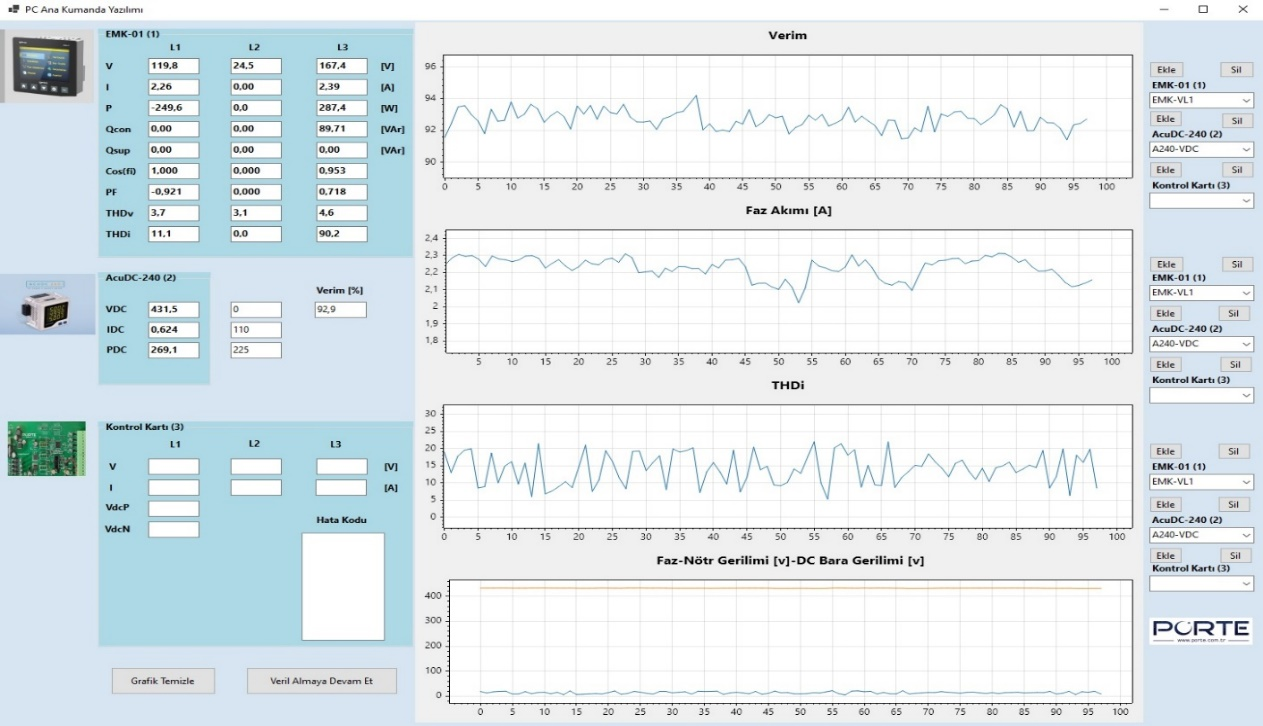
\includegraphics[width=0.98\textwidth]{deneysel/onceki_tez_sekil_5_16_klasik_pc.jpeg}
  \caption{\eskitezetiketi\ Klasik anahtarlama sırasında PC yazılımında alınan grafikler (önceki Şekil~5.16).}
  \label{fig:deney-eski-5-16}
  \label{fig:deney-klasik-kayitlar}
\end{figure}

Şekil~\ref{fig:deney-eski-5-17}'de yukarıdan aşağıya kontrol işareti, şebeke gerilimi, işlemciden alınan ortalama endüktör akımı ve akım probuyla ölçülen $L_1$ akımı bulunmaktadır. Kayıt, anahtarlama dalgalanmasını ve akımın sıfır çevresindeki davranışını doğrudan göstermektedir.

\begin{figure}[htbp]
  \centering
  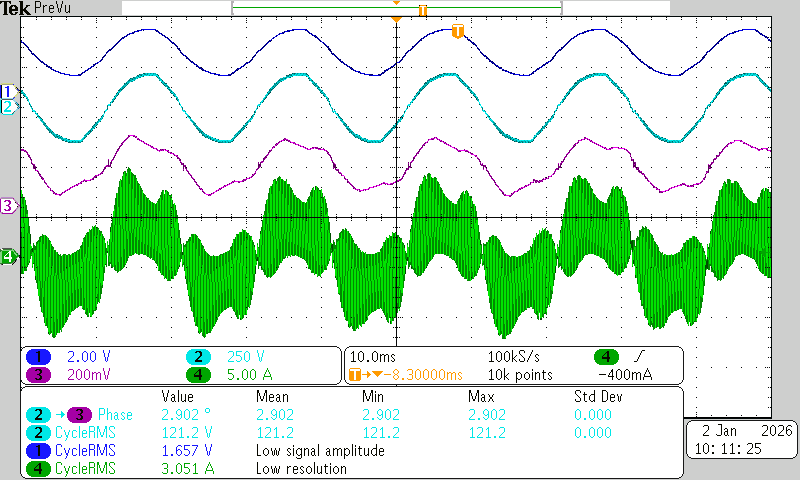
\includegraphics[width=0.94\textwidth]{deneysel/onceki_tez_sekil_5_17_klasik_l1.png}
  \caption{\eskitezetiketi\ Klasik yöntemde kontrol işareti, şebeke gerilimi, ortalama endüktör akımı ve $L_1$ akımı (önceki Şekil~5.17).}
  \label{fig:deney-eski-5-17}
\end{figure}

Şekil~\ref{fig:deney-eski-5-18}'de ilk üç kanal korunmuş, dördüncü kanalda faz akımı verilmiştir. $L_1$ akımı ile faz akımının ayrı kayıtlarda sunulması, filtre ve şebeke tarafındaki dalga biçimlerinin aynı fiziksel büyüklük olarak yorumlanmasını önlemektedir.

\begin{figure}[htbp]
  \centering
  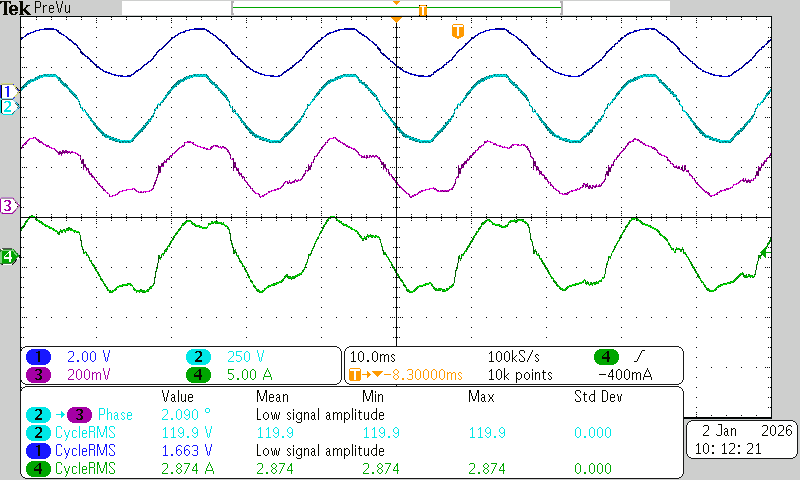
\includegraphics[width=0.94\textwidth]{deneysel/onceki_tez_sekil_5_18_klasik_faz.png}
  \caption{\eskitezetiketi\ Klasik yöntemde kontrol işareti, şebeke gerilimi, ortalama endüktör akımı ve faz akımı (önceki Şekil~5.18).}
  \label{fig:deney-eski-5-18}
\end{figure}

\section{Değiştirilmiş Anahtarlama Modu Deney Kayıtları}

Değiştirilmiş anahtarlama, yeni tezde nötr anahtar susturma yöntemi olarak adlandırılmıştır. İlgili yarım periyotta ters akım yolu kesilmekte, düşük görev oranında kesintili iletim ve üçüncü harmonik ağırlıklı akım zarfı ortaya çıkmaktadır. Önceki tez metni yüzde 94,2 verim, yüzde 46 akım THD'si, yaklaşık \SI{2.3}{\ampere} faz akımı, \SI{120}{\volt} faz--nötr gerilimi ve \SI{395}{\volt} DA bara gerilimi vermektedir.

\begin{figure}[htbp]
  \centering
  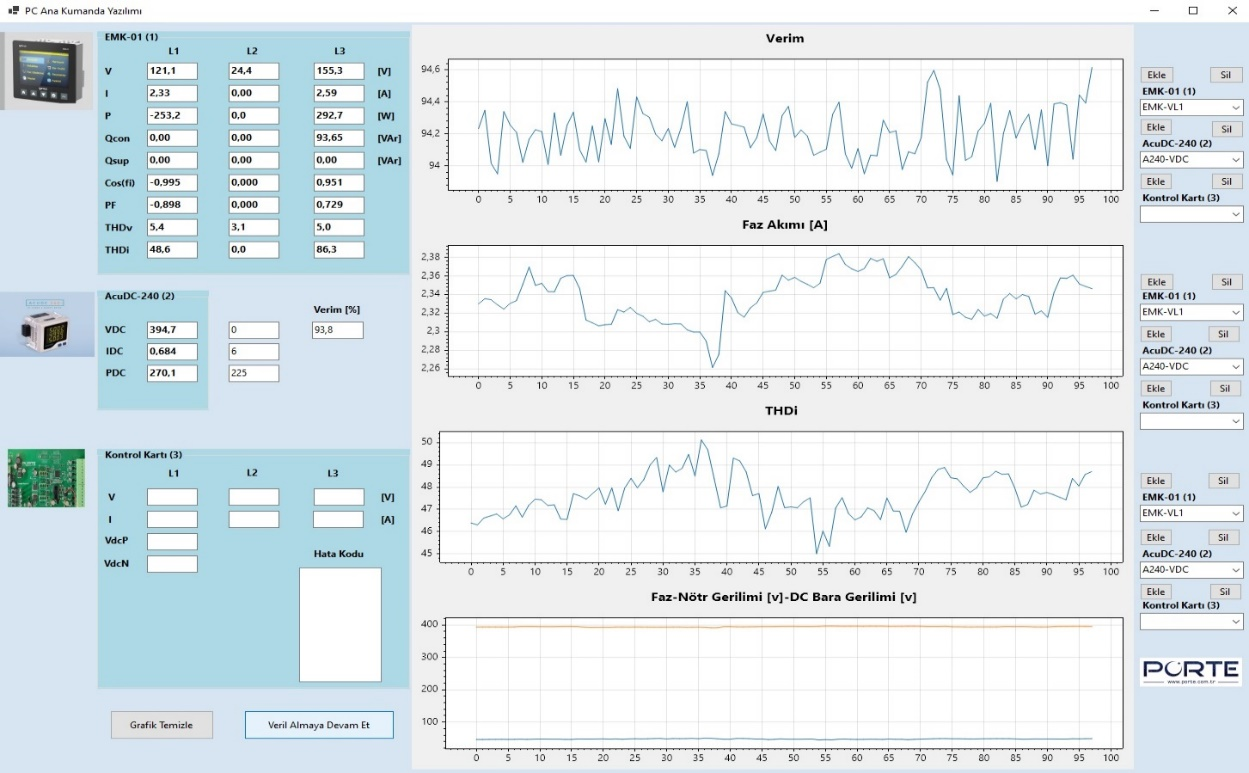
\includegraphics[width=0.98\textwidth]{deneysel/onceki_tez_sekil_5_19_susturma_pc.jpeg}
  \caption{\eskitezetiketi\ Değiştirilmiş anahtarlama modunda PC yazılımında elde edilen grafikler (önceki Şekil~5.19).}
  \label{fig:deney-eski-5-19}
  \label{fig:deney-susturma-kayitlar}
\end{figure}

Şekil~\ref{fig:deney-eski-5-20}, anahtarlamalı endüktör akımının sıfır çevresinde kesildiği aralıkları göstermektedir. Gözlenen zarf, Bölüm~\ref{chap:anahtarlama} içindeki Senaryo~2 ve üçüncü harmonik mekanizmasıyla nitel olarak uyumludur.

\begin{figure}[htbp]
  \centering
  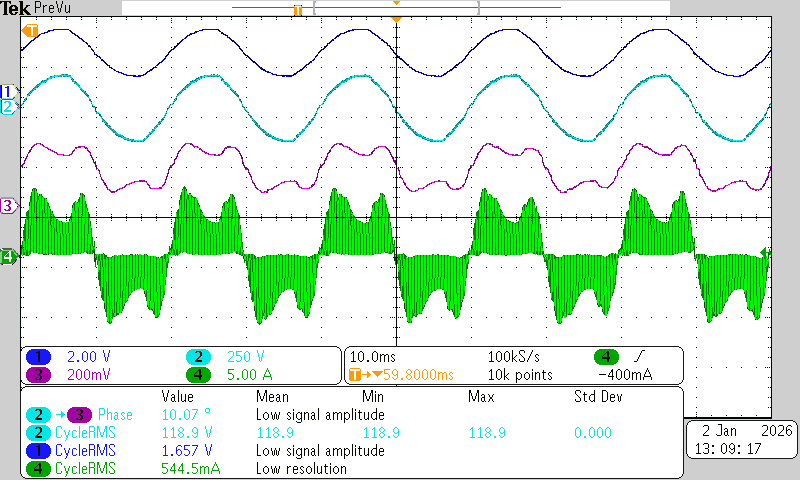
\includegraphics[width=0.94\textwidth]{deneysel/onceki_tez_sekil_5_20_susturma_l1.png}
  \caption{\eskitezetiketi\ Değiştirilmiş yöntemde kontrol işareti, şebeke gerilimi, ortalama endüktör akımı ve $L_1$ akımı (önceki Şekil~5.20).}
  \label{fig:deney-eski-5-20}
\end{figure}

Şekil~\ref{fig:deney-eski-5-21}, aynı yöntemin faz akımındaki belirgin biçim bozulmasını göstermektedir. Klasik yönteme göre farklı DA bara gerilimi kullanılması nedeniyle verim değişiminin tamamı yalnız anahtarlama yöntemine atfedilemez.

\begin{figure}[htbp]
  \centering
  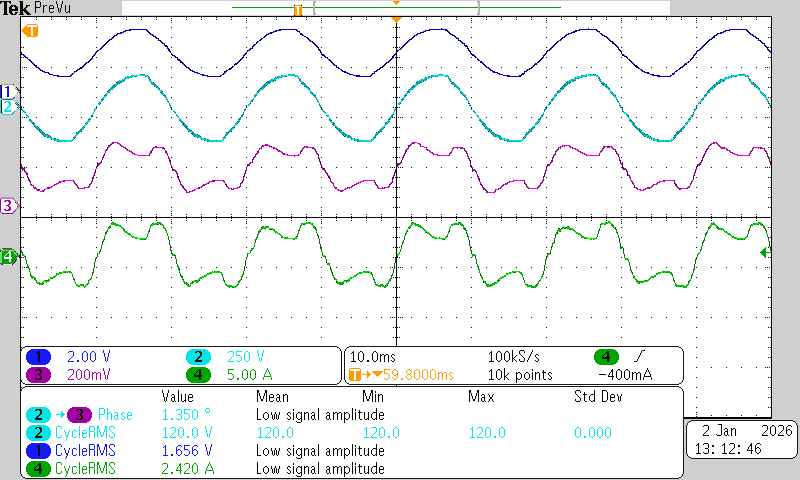
\includegraphics[width=0.94\textwidth]{deneysel/onceki_tez_sekil_5_21_susturma_faz.png}
  \caption{\eskitezetiketi\ Değiştirilmiş yöntemde kontrol işareti, şebeke gerilimi, ortalama endüktör akımı ve faz akımı (önceki Şekil~5.21).}
  \label{fig:deney-eski-5-21}
\end{figure}

\section{Değiştirilmiş Anahtarlama ve Sin\texorpdfstring{\textsuperscript{3}}{3} Deney Kayıtları}

Üçüncü yöntemde nötr anahtar susturma korunmuş ve akım zarfındaki harmonik bozulmayı azaltmak amacıyla Sin\textsuperscript{3} tabanlı terim eklenmiştir. Önceki tez metni yüzde 94,5 verim, yüzde 14 akım THD'si, yaklaşık \SI{2.3}{\ampere} faz akımı, \SI{124}{\volt} faz--nötr gerilimi ve \SI{427}{\volt} DA bara gerilimi bildirmektedir. Uygulanan terimin $K\sin^3(\theta)$ mı yoksa $K\sin(3\theta)$ mı olduğu kaynak kod bulunmadığından Bölüm~\ref{chap:sin3} içindeki açık doğrulama maddesi olarak korunmuştur.

\begin{figure}[htbp]
  \centering
  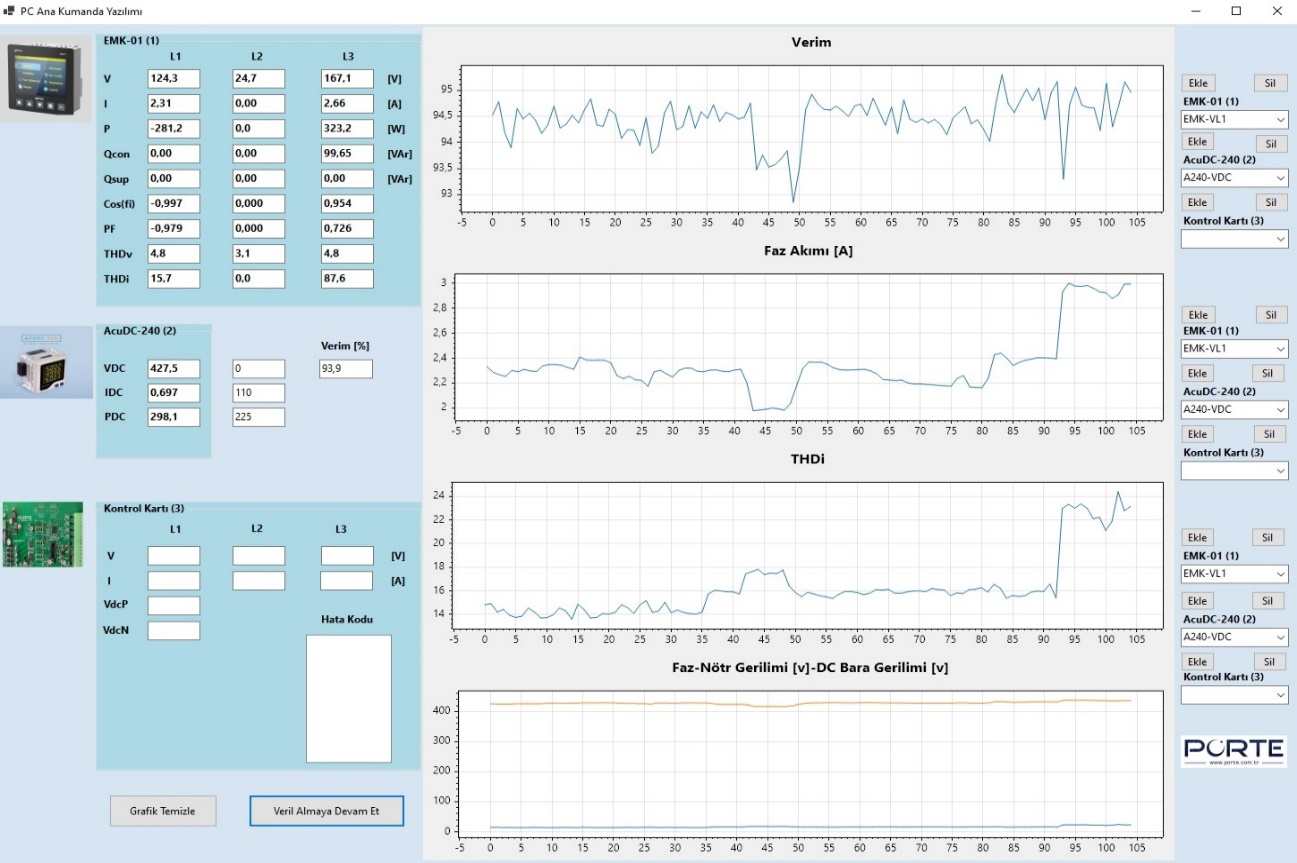
\includegraphics[width=0.98\textwidth]{deneysel/onceki_tez_sekil_5_22_sin3_pc.jpeg}
  \caption{\eskitezetiketi\ Sin\textsuperscript{3} uygulanmış değiştirilmiş anahtarlama modunda PC yazılımında alınan grafikler (önceki Şekil~5.22).}
  \label{fig:deney-eski-5-22}
  \label{fig:deney-sin3-kayitlar}
\end{figure}

Şekil~\ref{fig:deney-eski-5-23}, susturma deneyine göre daha düzenli bir $L_1$ akım zarfı göstermektedir. Nitel iyileşme, önceki tezde bildirilen THD azalmasıyla uyumludur.

\begin{figure}[htbp]
  \centering
  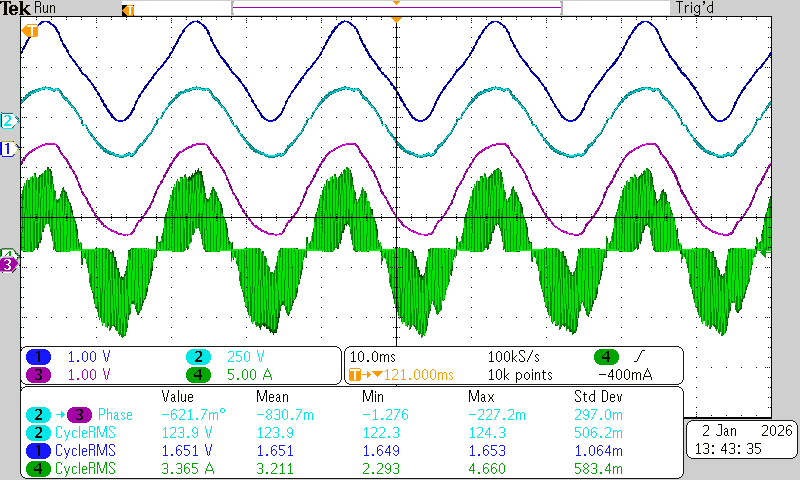
\includegraphics[width=0.94\textwidth]{deneysel/onceki_tez_sekil_5_23_sin3_l1.png}
  \caption{\eskitezetiketi\ Sin\textsuperscript{3} uygulanmış yöntemde kontrol işareti, şebeke gerilimi, ortalama endüktör akımı ve $L_1$ akımı (önceki Şekil~5.23).}
  \label{fig:deney-eski-5-23}
\end{figure}

Şekil~\ref{fig:deney-eski-5-24}, faz akımındaki zarfın değiştirilmiş anahtarlamaya göre düzeldiğini göstermektedir. Klasik ve Sin\textsuperscript{3} deneyleri farklı DA bara ve faz gerilimlerinde yapıldığından tek değişkenli nedensel üstünlük sonucu çıkarılmamıştır.

\begin{figure}[htbp]
  \centering
  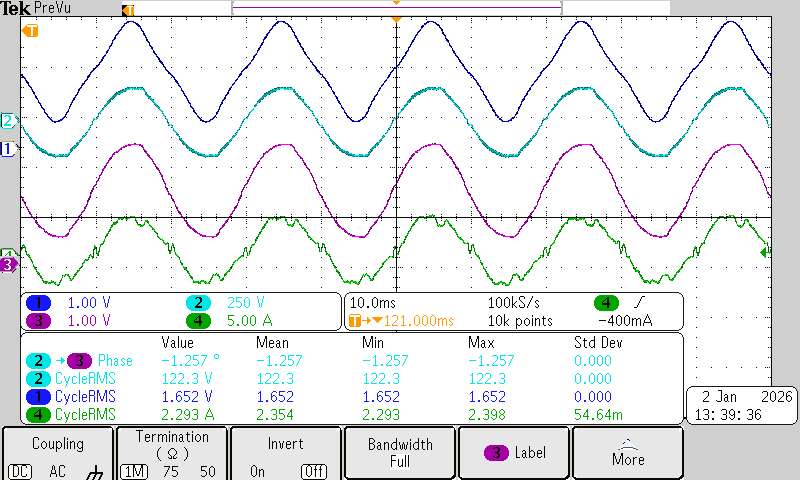
\includegraphics[width=0.94\textwidth]{deneysel/onceki_tez_sekil_5_24_sin3_faz.png}
  \caption{\eskitezetiketi\ Sin\textsuperscript{3} uygulanmış yöntemde kontrol işareti, şebeke gerilimi, ortalama endüktör akımı ve faz akımı (önceki Şekil~5.24).}
  \label{fig:deney-eski-5-24}
\end{figure}

\section{Önceki Deney Sonuçları Tablosu}

Önceki tez, deney ve simülasyon sonuçlarını Tablo~5.4'te birlikte karşılaştırdığını belirtmektedir. Kaynak Word tablosundaki gerçek uygulama hücreleri dolu, simülasyon hücreleri ise boştur. Tablo~\ref{tab:deney-dusuk-guc-ozeti}, söz konusu yapıyı boş hücreler dahil korumaktadır; eksik simülasyon değerleri tahminle doldurulmamıştır.

\begin{table}[htbp]
  \centering
  \caption{\eskitezetiketi\ Deneysel ve simülasyon çalışmaları sonucunda elde edilen verim ve THD değerlerinin üç yaklaşım ile karşılaştırılması; önceki Tablo~5.4'ün dolu ve boş hücreleri korunmuştur.}
  \label{tab:deney-dusuk-guc-ozeti}
  \label{tab:deney-eski-5-4}
  \footnotesize
  \begin{tabularx}{\textwidth}{p{0.28\textwidth} >{\centering\arraybackslash}X >{\centering\arraybackslash}X >{\centering\arraybackslash}X >{\centering\arraybackslash}X}
    \toprule
    & \multicolumn{2}{c}{Gerçek uygulama sonuçları} & \multicolumn{2}{c}{Simülasyon sonuçları} \\
    \cmidrule(lr){2-3}\cmidrule(lr){4-5}
    Yöntem & Verim & THD$_i$ (L1) & Verim & THD$_i$ (L1) \\
    \midrule
    Complement anahtarlama & \%92,50 & \%15 & & \\
    Değiştirilmiş anahtarlama & \%94,20 & \%46 & & \\
    Sinküp uygulanmış değiştirilmiş anahtarlama & \%94,50 & \%14 & & \\
    \bottomrule
  \end{tabularx}
\end{table}

Çevre metin klasik yöntemde yüzde 90,45 ve önerilen yöntemde yaklaşık yüzde 93 simülasyon verimi bildirmektedir; yöntem bazındaki simülasyon THD değerleri ile üçüncü yöntemin açık simülasyon verimi aynı tabloda bulunmamaktadır. Sayısal karşılaştırma Bölüm~\ref{chap:anahtarlama} ve Bölüm~\ref{chap:sin3} içindeki gerçek model çıktıları yeniden üretildiğinde tamamlanacaktır.

\tezcalismanotu{D6-3 --- Simülasyon--deney karşılaştırması}{Bölüm~\ref{chap:anahtarlama} ve Bölüm~\ref{chap:sin3} için doğrulanmış model çıktıları elde edildiğinde klasik, nötr susturma ve susturma+Sin\textsuperscript{3} yöntemleri aynı DA bara, şebeke gerilimi, akım referansı ve analiz penceresinde karşılaştırılacaktır. Tablo~\ref{tab:deney-dusuk-guc-ozeti} içindeki boş simülasyon hücreleri tahminle doldurulmayacak; yeni sonuçlar ayrı ve kaynak koşu kimliği bulunan bir tabloda verilecektir.}

\section{Kaynak İçi Doğrulama ve Jüri Talebi}

\begin{figure}[htbp]
  \centering
  \begin{tikzpicture}[
    node distance=8mm and 10mm,
    block/.style={draw=blue!55!black,fill=blue!7,rounded corners,align=center,minimum height=10mm,text width=28mm,font=\small},
    meas/.style={draw=green!50!black,fill=green!8,rounded corners,align=center,minimum height=10mm,text width=28mm,font=\small},
    data/.style={draw=orange!70!black,fill=orange!10,rounded corners,align=center,minimum height=10mm,text width=30mm,font=\small},
    arr/.style={-{Latex[length=2.5mm]},thick}
  ]
    \node[block] (dc) {DA bara\\AcuDC240 + şönt};
    \node[block,right=of dc] (inv) {T-tipi evirici\\LCL filtre};
    \node[block,right=of inv] (grid) {Varyak ve\\AA şebeke};
    \draw[arr] (dc) -- node[above,font=\scriptsize] {$P_{dc}$} (inv);
    \draw[arr] (inv) -- node[above,font=\scriptsize] {$v_g,i_g$} (grid);
    \node[meas,below=of inv] (scope) {Osiloskop\\$i_{L1}$, $i_g$, $v_g$, DAC};
    \node[meas,below=of grid] (ac) {EMK-01 + CT\\$P_{ac}$, THD, PF};
    \node[meas,below=of dc] (ctrl) {Kontrol/ölçüm kartı\\ADC, PWM, FAULT};
    \draw[arr] (inv) -- (scope);
    \draw[arr] (grid) -- (ac);
    \draw[arr] (inv) -- (ctrl);
    \node[data,below=15mm of scope] (pc) {PC ana kumanda yazılımı\\RS485/Modbus RTU};
    \draw[arr] (ctrl) -- (pc);
    \draw[arr] (ac) -- (pc);
    \draw[arr] (dc) |- (pc);
    \draw[arr,dashed] (scope) -- node[right,font=\scriptsize] {ekran kaydı} (pc);
  \end{tikzpicture}
  \caption{\juriistegietiketi\ Deney düzeneğindeki güç, ölçüm ve veri toplama akışı; önceki tez açıklamalarından yeniden düzenlenmiştir.}
  \label{fig:deney-olcum-zinciri}
\end{figure}

Tablo~\ref{tab:olcum-cihazlari}, önceki tezde bildirilen cihaz ve sensörleri doğrulama sınırlarıyla birlikte toplamaktadır. Kaynak içindeki ``Class 0,1'' ve AcuDC240 yüzde hata değerleri aynı şey olarak kabul edilmemiş; osiloskop için yazılan ``300 Hz'' ifadesi model ailesiyle uyuşmadığından üretici belgesi bekleyen kayıt olarak işaretlenmiştir.

\begin{table}[htbp]
  \centering
  \caption{\eskitezetiketi\ \juriistegietiketi\ Önceki tezde bildirilen ölçüm cihazları ve doğrulama sınırları.}
  \label{tab:olcum-cihazlari}
  \footnotesize
  \begin{tabularx}{\textwidth}{p{0.19\textwidth} p{0.23\textwidth} p{0.20\textwidth} X}
    \toprule
    Büyüklük & Cihaz / sensör & Bildirilen özellik & Doğrulama notu \\
    \midrule
    AA güç ve THD & Entes EMK-01 ve 50/5 oranlı, \SI{5}{\volt\ampere} akım transformatörleri & Class 0.1 & Kalibrasyon belgesinin Ek A'da olduğu yazılmış; bağımsız belge mevcut klasörde bulunmamaktadır. \\
    DA güç & Accuenergy AcuDC240 ve \SI{20}{\ampere}/\SI{60}{\milli\volt} şönt & Akım/gerilim yüzde 0,2; güç/enerji yüzde 0,5 & Bölüm girişindeki ``Class 0,1'' ifadesiyle uyuşmazlık üretici belgesiyle kesinleştirilecektir. \\
    Hızlı akım & Tektronix TCP0150 & \SI{150}{\ampere}, \SI{20}{\mega\hertz} & Prob oranı ham osiloskop dosyasıyla doğrulanacaktır. \\
    Hızlı gerilim & Tektronix THDP0200 & \SI{1500}{\volt}, \SI{200}{\mega\hertz} & Kanal zayıflatması ve ortak-mod sınırı ham kayıtla doğrulanacaktır. \\
    Osiloskop & Tektronix DPO3034 & Kaynakta ``300 Hz, 2,5 GS/s'' & ``300 Hz'' ifadesi model veri sayfasıyla uyuşmadığından bant genişliği doğrulanmalıdır. \\
    Faz/LCL akımı & HLSR 20-P/SP33 & \SI{23}{\milli\volt\per\ampere}; \SI{39.9}{\ampere} RMS hesap sınırı & Kazanç ve ADC ölçekleme katsayıları kontrol koduyla doğrulanacaktır. \\
    Gerilim ölçümü & AMC1200 tabanlı izole kart & Kazanç 8; \SI{2.6}{\volt} ADC aralığı & Direnç oranı ve kanal kalibrasyonu şemadan doğrulanacaktır. \\
    \bottomrule
  \end{tabularx}
\end{table}

\tezcalismanotu{D6-4 --- Cihaz belgeleri ve kanal ölçekleri}{AcuDC240, EMK-01, DPO3034, TCP0150, THDP0200, HLSR 20-P/SP33 ve AMC1200 için üretici veri sayfası atıfları eklenecektir. Kullanılan cihaz seri numarası, geçerli kalibrasyon belgesi, osiloskop kanal zayıflatması, prob oranı, akım transformatörü oranı ve ADC ölçekleme katsayısı bulunabiliyorsa Ek~A'da verilecektir.}

\tezcalismanotu{D6-5 --- Ölçüm belirsizliği}{DA giriş ve AA çıkış gücünün cihaz doğrulukları, şönt/akım transformatörü oranları ve kanal ölçekleme belirsizlikleri kullanılarak birleşik verim belirsizliği hesaplanacaktır. Bağımsız belirsizlikler için ilk yaklaşım
\[
u_{\eta}=\eta\sqrt{\left(\frac{u_{P_{ac}}}{P_{ac}}\right)^2+\left(\frac{u_{P_{dc}}}{P_{dc}}\right)^2}
\]
olacaktır. Nihai tabloda verim değerleri belirsizlik aralığıyla birlikte raporlanacaktır.}

\begin{table}[htbp]
  \centering
  \caption{\eskitezetiketi\ \juriistegietiketi\ Üç yöntem için önceki tez metninde bildirilen çalışma koşulları.}
  \label{tab:deney-kosullari}
  \footnotesize
  \begin{tabularx}{\textwidth}{p{0.21\textwidth} *{3}{>{\centering\arraybackslash}X} X}
    \toprule
    Büyüklük & Klasik & Nötr susturma & Susturma+Sin\textsuperscript{3} & Yorum \\
    \midrule
    Faz akımı & \SI{2.3}{\ampere} & \SI{2.3}{\ampere} & \SI{2.3}{\ampere} & Düşük güç noktası; anma testi değildir. \\
    Faz--nötr gerilimi & \SI{120}{\volt} & \SI{120}{\volt} & \SI{124}{\volt} & Yöntemler tam aynı gerilimde değildir. \\
    DA bara gerilimi & \SI{430}{\volt} & \SI{395}{\volt} & \SI{427}{\volt} & Yöntemler tam aynı bara koşulunda değildir. \\
    Güç faktörü & $-0{,}990$--$1{,}000$ & $-0{,}995$ & $-0{,}997$ & İşaret, güç akış yönü konvansiyonundan etkilenmektedir. \\
    \bottomrule
  \end{tabularx}
\end{table}

\tezcalismanotu{D6-6 --- Tekrarlanabilirlik}{Aynı çalışma noktasında her yöntem için tercihen en az üç bağımsız kayıt alınacak; verim, THD, RMS akım ve güç faktörü sonuçları ortalama, standart sapma ve gözlem sayısıyla raporlanacaktır. Tek kayıtla sınırlı tarihsel sonuçlarda istatistiksel üstünlük iddiası kurulmayacaktır.}

\tezcalismanotu{D6-7 --- Eşit koşullarda yöntem karşılaştırması}{Klasik, nötr susturma ve susturma+Sin\textsuperscript{3} yöntemlerinin karşılaştırılmasında DA bara gerilimi, faz--nötr gerilimi, akım/güç referansı, anahtarlama frekansı, denetleyici, sıcaklık ve analiz penceresi sabit tutulacaktır. Mevcut kayıtlar farklı bara ve faz gerilimlerine sahip olduğundan nedensel verim üstünlüğü yalnız yeni ortak koşullu testten sonra savunulacaktır.}

Önceki tez paragraflarındaki özet değerlerle PC ekranlarında görünen anlık değerler aynı değildir. Tablo~\ref{tab:deney-metin-ekran-karsilastirma}, farkları görünür kılmaktadır. Ekran değeri, görselde L1 sütununda ve DA analizörü alanında okunabilen tek anlık görüntü; metin değeri ise önceki tez yazarının deney özeti olarak korunmuştur.

\begin{table}[htbp]
  \centering
  \caption{\eskitezetiketi\ \juriistegietiketi\ Önceki tez metni ile PC ekranlarında okunabilen anlık değerlerin karşılaştırılması.}
  \label{tab:deney-metin-ekran-karsilastirma}
  \footnotesize
  \begin{tabularx}{\textwidth}{p{0.21\textwidth} p{0.16\textwidth} >{\centering\arraybackslash}X >{\centering\arraybackslash}X X}
    \toprule
    Yöntem & Büyüklük & Metin özeti & PC ekranı & Farkın durumu \\
    \midrule
    Klasik & Verim & \%92,5 & \%92,9 & Ortalama/anlık ayrımı doğrulanamadı. \\
    Klasik & THD$_i$ & \%15 & \%11,1 & Analiz penceresi ve ortalama yöntemi eksik. \\
    Klasik & $V_{dc}$ & \SI{430}{\volt} & \SI{431.5}{\volt} & Yakın değerler. \\
    \midrule
    Nötr susturma & Verim & \%94,2 & \%93,8 & Ortalama/anlık ayrımı doğrulanamadı. \\
    Nötr susturma & THD$_i$ & \%46 & \%48,6 & Aynı yüksek bozulma eğilimi; sayısal fark açık. \\
    Nötr susturma & $V_{dc}$ & \SI{395}{\volt} & \SI{394.7}{\volt} & Yakın değerler. \\
    \midrule
    Susturma+Sin\textsuperscript{3} & Verim & \%94,5 & \%93,9 & Ortalama/anlık ayrımı doğrulanamadı. \\
    Susturma+Sin\textsuperscript{3} & THD$_i$ & \%14 & \%15,7 & Aynı iyileşme eğilimi; sayısal fark açık. \\
    Susturma+Sin\textsuperscript{3} & $V_{dc}$ & \SI{427}{\volt} & \SI{427.5}{\volt} & Yakın değerler. \\
    \bottomrule
  \end{tabularx}
\end{table}

Ham PC/Modbus ve osiloskop kayıtları bulunmadan farklı değerlerin ortalama, medyan, seçilmiş an veya farklı faz sonucu olup olmadığı belirlenemez. Tablo~\ref{tab:deney-metin-ekran-karsilastirma} hata düzeltme tablosu değil, kaynak içi tutarlılık denetimidir.

Jürinin düşük, orta ve nominal güçte aynı kapalı çevrim yapının karşılaştırılması talebi mevcut deneylerle bütünüyle karşılanmamaktadır. Önceki tez yalnız yaklaşık \SI{2.3}{\ampere} düşük güç noktasını belgelemekte; orta ve nominal güç için aynı ölçüm seti bulunmamaktadır. Tablo~\ref{tab:deney-juri-durum}, mevcut kanıt ile tamamlanması gereken doğrulamayı ayırmaktadır.

\begin{table}[htbp]
  \centering
  \caption{\juriistegietiketi\ Deneysel doğrulamanın jüri talebine göre yeterlilik durumu.}
  \label{tab:deney-juri-durum}
  \small
  \begin{tabularx}{\textwidth}{p{0.19\textwidth} p{0.23\textwidth} X X}
    \toprule
    Çalışma bölgesi & Mevcut kanıt & Eksik doğrulama & Tezdeki kullanım \\
    \midrule
    Düşük güç & Üç yönteme ait PC ve osiloskop ekranları; metin özeti & Ham zaman serisi, ortak bara/şebeke koşulu, tekrar ve belirsizlik & Önceki tezden aktarılan deneysel destekleyici kanıt \\
    Orta güç & Kayıt bulunamadı & Aynı kontrol ve ölçüm zinciriyle en az üç tekrar & Sonuç iddiası kurulmayacak \\
    Nominal / erişilebilir en yüksek güç & Kayıt bulunamadı & Güvenlik sınırı, termal durum, doyum, THD ve verim & Jüri talebi açık eksik olarak gösterilecek \\
    Geçici rejim & Kayıt bulunamadı & Referans basamağı, şebeke değişimi ve kompanzasyon aç/kapa geçişi & Gelecek doğrulama veya sınırlılık \\
    \bottomrule
  \end{tabularx}
\end{table}

\tezcalismanotu{D6-8 --- Düşük, orta ve nominal güç doğrulaması}{Jüri talebi doğrultusunda aynı kapalı çevrim ve ölçüm zinciri düşük, orta ve güvenli biçimde erişilebilen en yüksek/nominal güç noktalarında çalıştırılacaktır. Her noktada DA/AA güç, verim, THD, güç faktörü, RMS akım, doyum, anahtarlama davranışı ve termal durum aynı tablo biçiminde raporlanacaktır. Yeni test yapılamazsa orta ve nominal güç için deneysel sonuç iddiası kurulmayacaktır.}

\tezcalismanotu{D6-9 --- Geçici rejim deneyleri}{Kararlı durum kayıtlarına ek olarak akım veya güç referansı basamağı, şebeke gerilimi değişimi ve Sin\textsuperscript{3} kompanzasyonunun açma/kapama geçişi incelenecektir. Yerleşme süresi, aşım, doyum süresi, akım kalitesi ve koruma davranışı raporlanacak; hızlı geçici rejimler eşzamanlı osiloskop kanallarıyla kaydedilecektir.}

\subsection{Sonradan Gelen Çalışma Kitabının Sayısal Denetimi}

2026-08-17 tarihli çalışma kitabının ``Gerçek uygulama sonuçları'' alanı Senaryo~1--3 için tek satırlık özetler içermekte, ham zaman serisi veya tekrar koşusu vermemektedir. Tablo~\ref{tab:gelen-excel-senaryolar}, hücrelerdeki değerleri değiştirmeden ve $\eta_{VI}=100P_{\mathrm{out}}/(V_{\mathrm{dc}}I_{\mathrm{dc}})$ bağımsız hesabını ayrıca göstererek kaynağın izini korumaktadır.

\begin{table}[htbp]
  \centering
  \caption{2026-08-17 tarihli çalışma kitabındaki gerçek uygulama özeti ve DA giriş çarpımından yeniden hesaplanan verim.}
  \label{tab:gelen-excel-senaryolar}
  \footnotesize
  \begin{tabularx}{\textwidth}{c r r r r r r r}
    \toprule
    Senaryo & $V_{dc}$ (V) & $I_{dc}$ (A) & $V_{ac}$ (V RMS) & $I_{faz}$ (A) & $P_o$ (W) & THD (\%) & $\eta_{VI}$ (\%) \\
    \midrule
    1 & 431,5 & 0,624 & 119,8 & 2,26 & 249,6 & 15 & 92,700 \\
    2 & 395,0 & 0,684 & 121,0 & 2,33 & 253,2 & 47 & 93,715 \\
    3 & 427,5 & 0,697 & 124,3 & 2,31 & 281,2 & 14 & 94,373 \\
    \bottomrule
  \end{tabularx}
\end{table}

Çalışma kitabındaki bildirilen verimler sırasıyla \%92,5, \%94,2 ve \%94,5'tir. Yeniden hesaplanan değerlerle farklar yaklaşık $-0{,}20$, $+0{,}48$ ve $+0{,}13$ yüzde puandır. Farkların yuvarlama, farklı ortalama penceresi veya ek kayıp teriminden kaynaklanıp kaynaklanmadığı ham güç örnekleri olmadan çözülemez. Ayrıca kitabın ``simülasyon'' satırları aynı temel sayıları tekrar etmekte; bağımsız Simulink çıktısı veya ham iz sağlamamaktadır. Bu nedenle tablo deneysel özet olarak kullanılmış, simülasyon doğrulaması sayılmamıştır.

\section{Bölüm Sonucu}

Önceki tezdeki deney bölümünün şekil, tablo ve kavram zinciri eksiksiz aktarılmıştır. Deney düzeneği; T-tipi güç katı, faz modülleri, kontrol/buffer/sürücü kartları, gerilim ve akım ölçüm devreleri, koruma devresi, AA ve DA analizörleri, şönt bağlantısı, PC yazılımı ve üç yönteme ait ekran kayıtlarıyla birlikte sunulmuştur. Şekil üzerindeki numaralar ile Tablo~6.1--6.3 arasındaki özgün ilişkiler korunmuştur.

Üç yönteme ait kayıtlar, nötr susturmanın düşük güçte verimi artırırken harmonik bozulmayı büyüttüğü; Sin\textsuperscript{3} teriminin ise söz konusu bozulmayı azalttığı yönündeki mekanizmayı nitel olarak desteklemektedir. Sayısal sonuçların kanıt düzeyi kaynak içi tutarlılık denetimiyle sınırlandırılmıştır. Metin ile ekran değerleri arasındaki farklar, çalışma kitabındaki boş/tekrarlı simülasyon hücreleri, DA giriş çarpımından yeniden hesaplanan verim farkları, yöntemler arasındaki DA bara/şebeke gerilimi değişimi ve ham kayıt yokluğu açıkça gösterilmiştir. Jürinin nominal güçte kapalı çevrim ve karşılaştırmalı deney talebi mevcut arşivle tamamlanmış sayılmamıştır.
